  \begin{figure*}%[tbp]
  %\begin{minipage}{0.48\linewidth}
          \begin{minipage}{0.65\linewidth}
            \centering
            {Calibrated classifier score $f_j$}
            \\
            \vspace{2mm}
            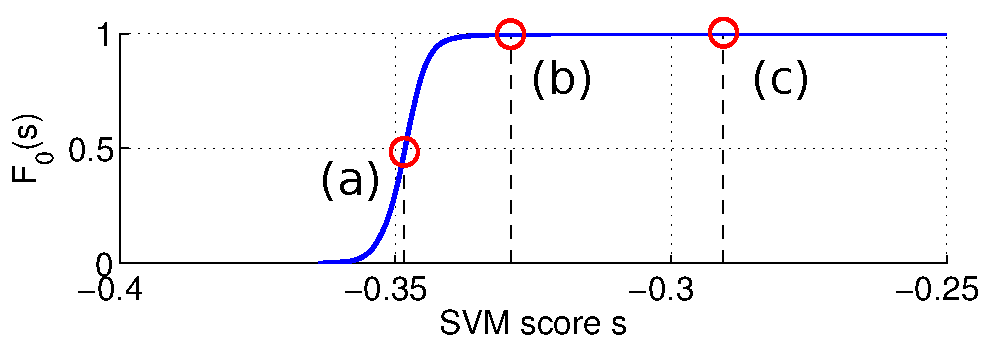
\includegraphics[width=\linewidth]{imgs/wVS3q/2882/graphBigO.pdf}
          \end{minipage} 
          %
          \begin{minipage}{\wii}
            \centering
            \centerline{Target database image $j$}
            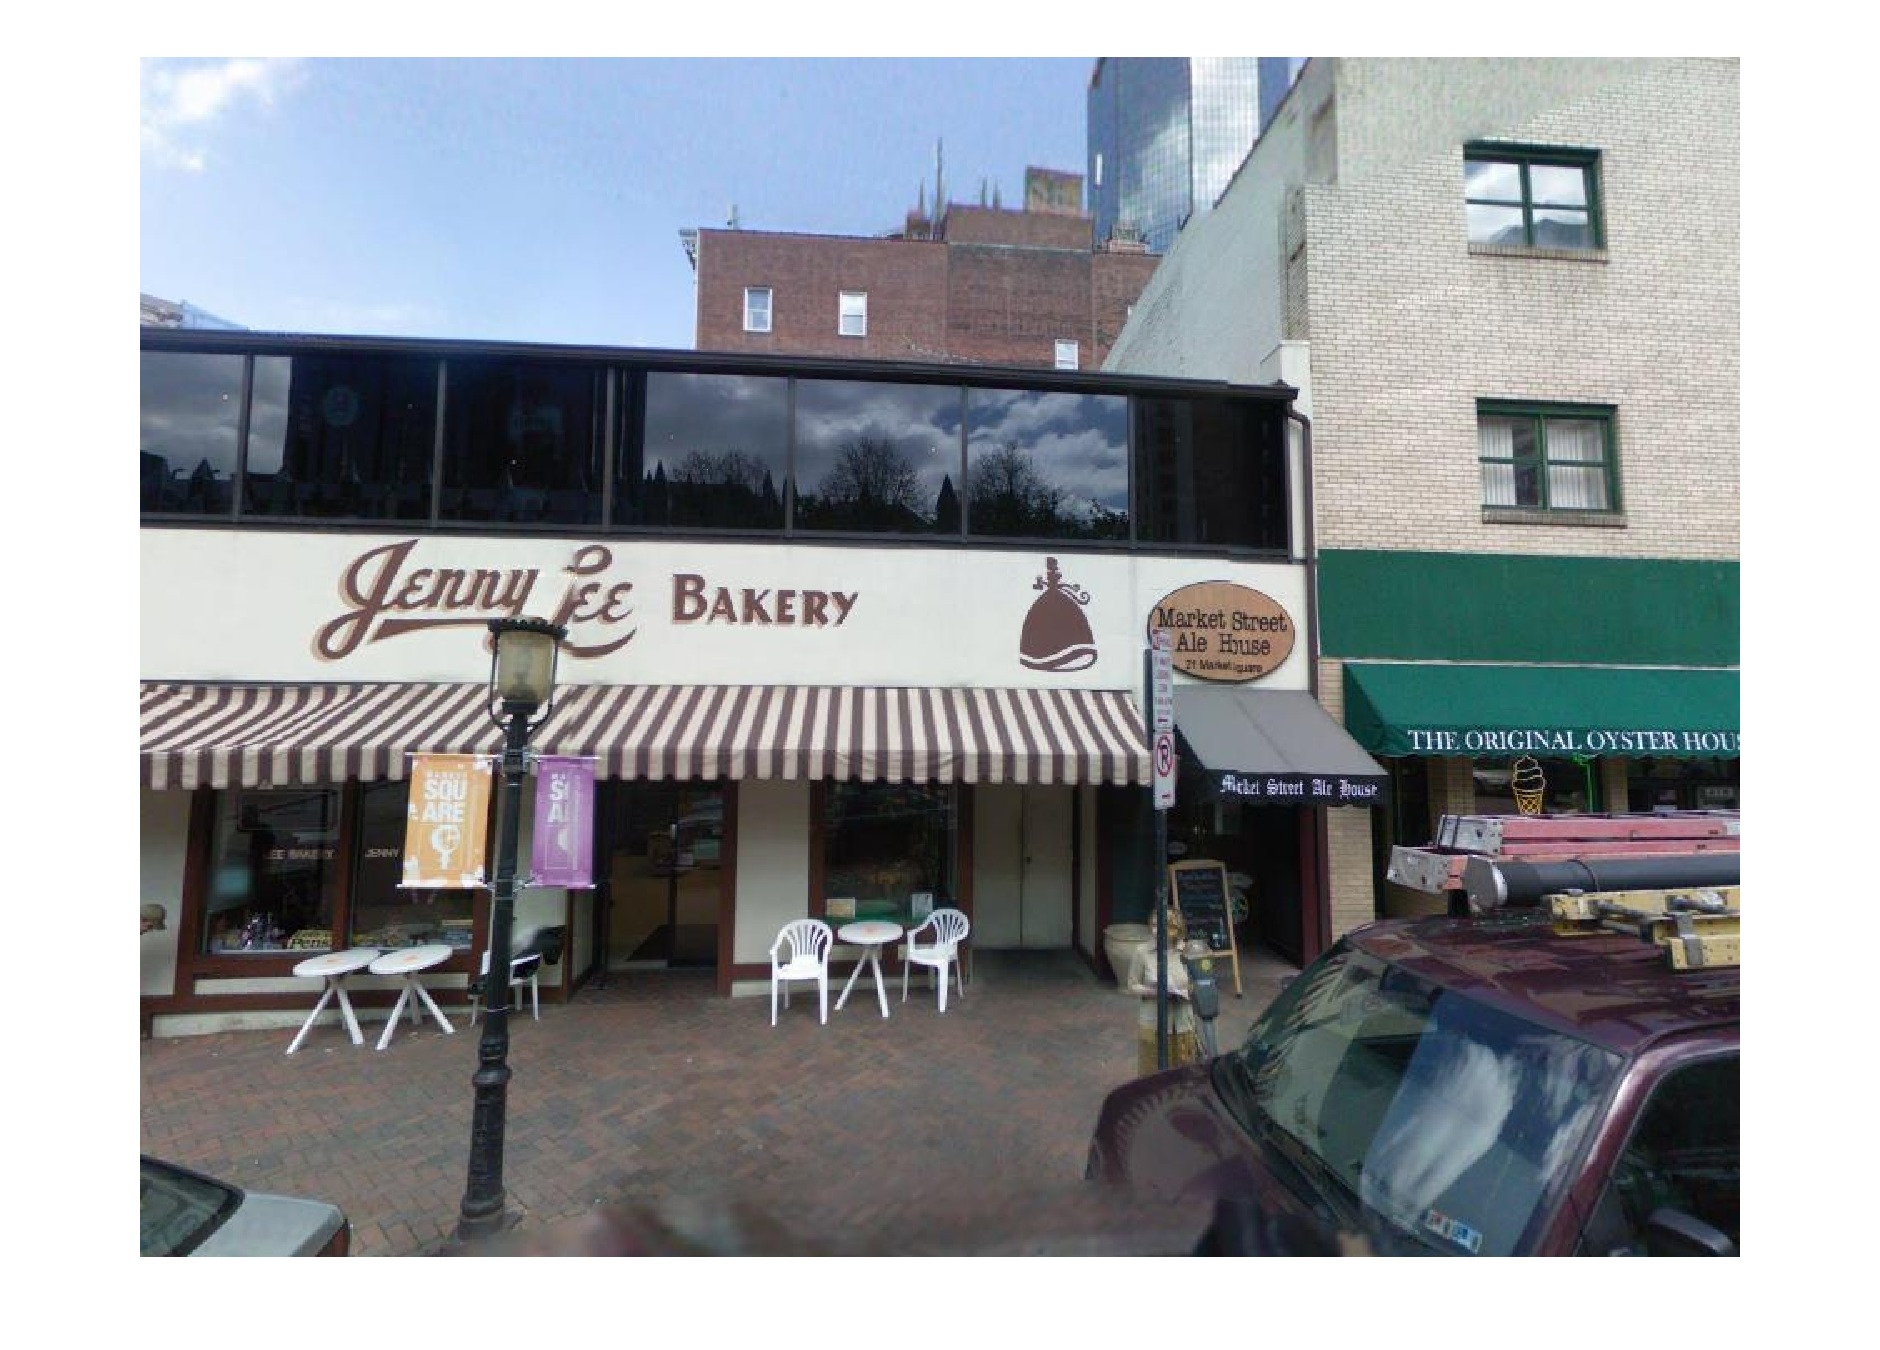
\includegraphics[width=\linewidth]{imgs/wVS3q/2882/j.jpg}
          \end{minipage}  
          \vspace{3mm}
          \\
          \centerline{Classified query images $f_j(q)$} 
          \\
          \begin{minipage}{\wii}
            \centering
            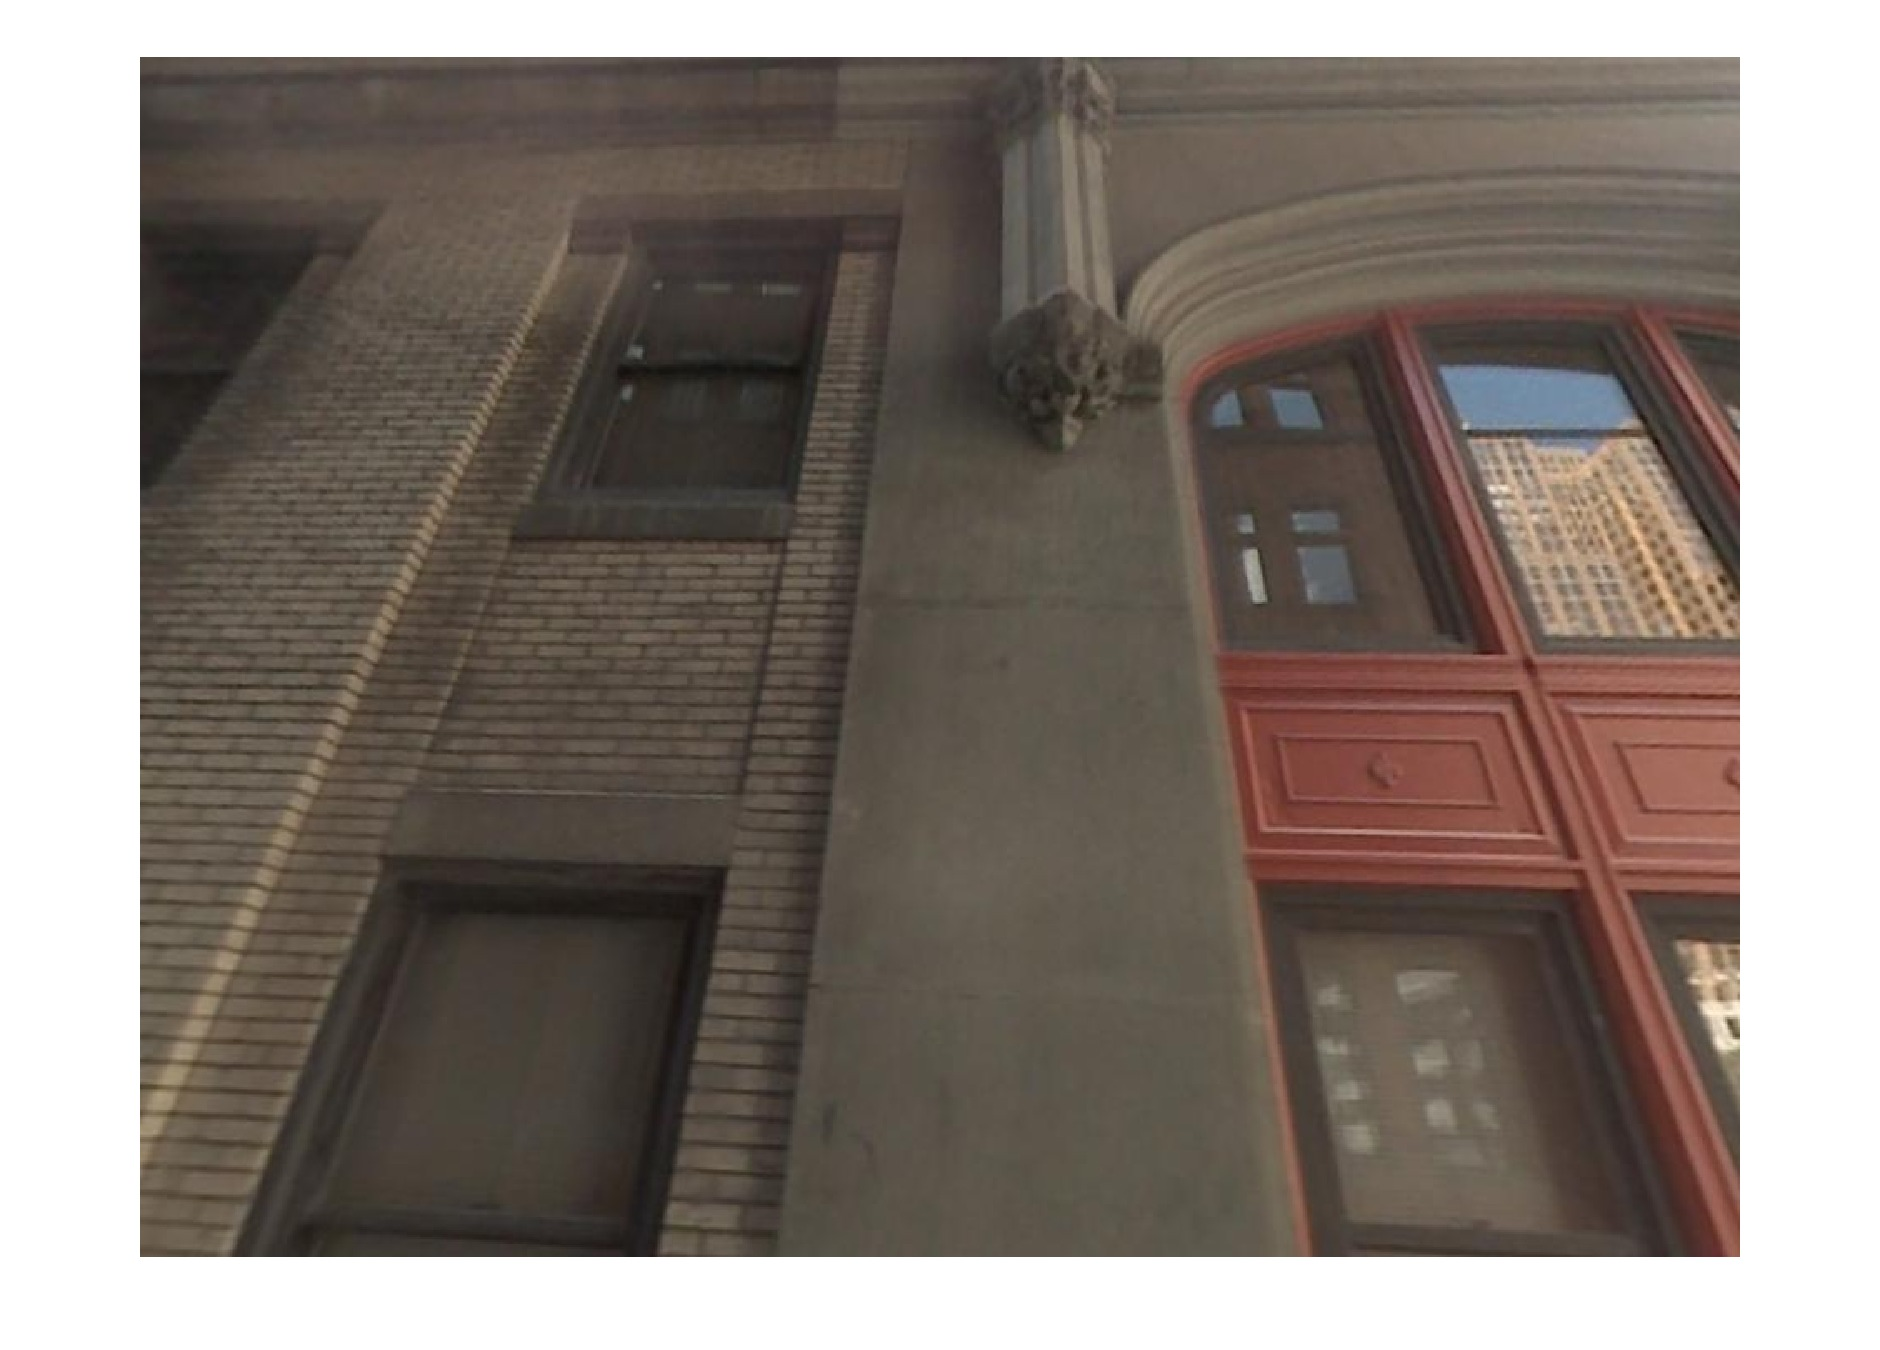
\includegraphics[width=\linewidth]{imgs/wVS3q/2882/a.jpg}
          \end{minipage}
          %  
          \begin{minipage}{\wii}
            \centering
            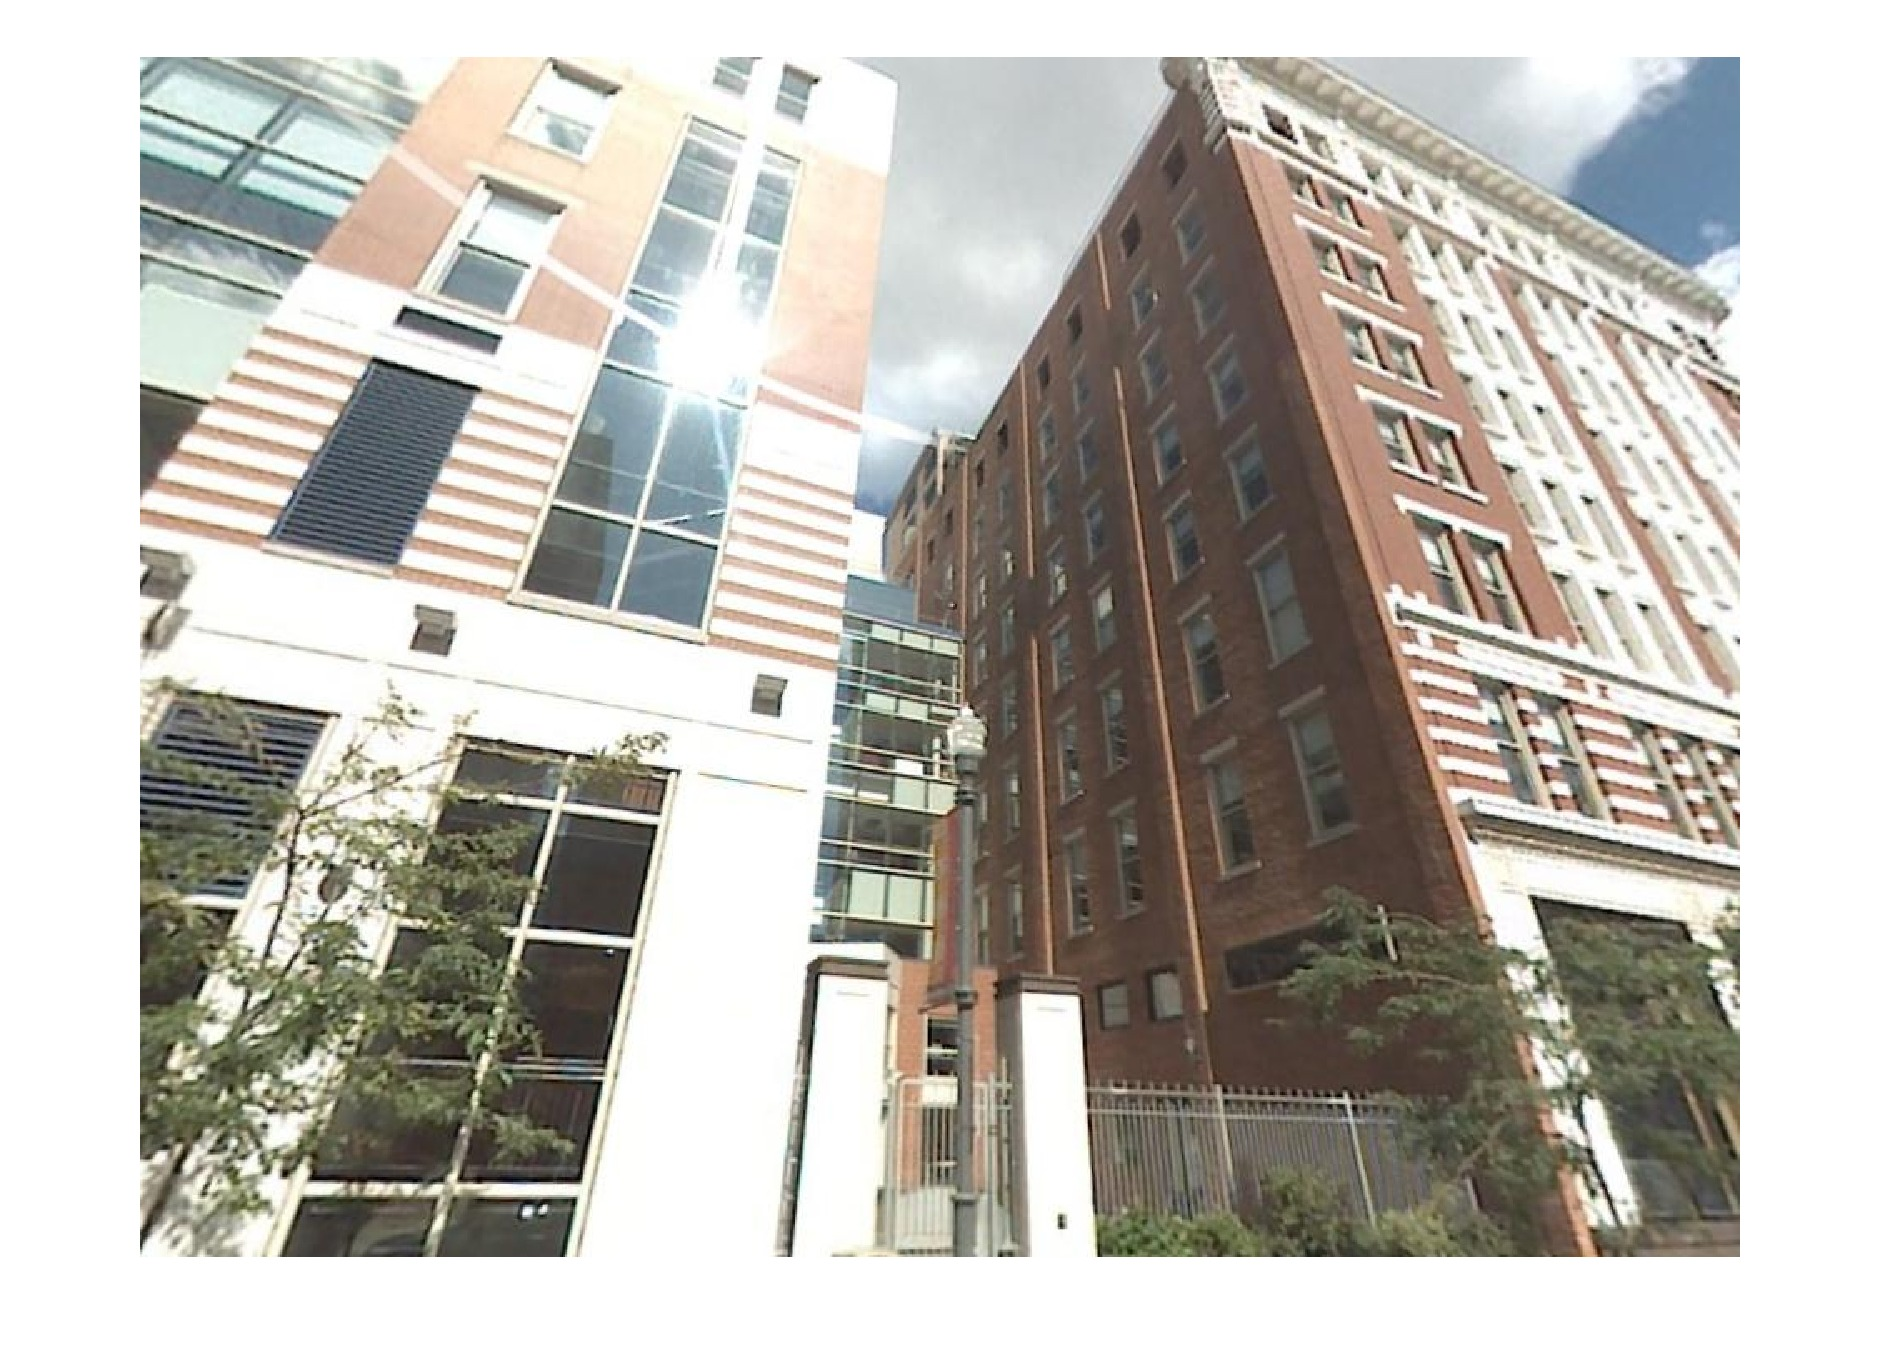
\includegraphics[width=\linewidth]{imgs/wVS3q/2882/b.jpg}
          \end{minipage}
          %  
          \begin{minipage}{\wii}
            \centering
            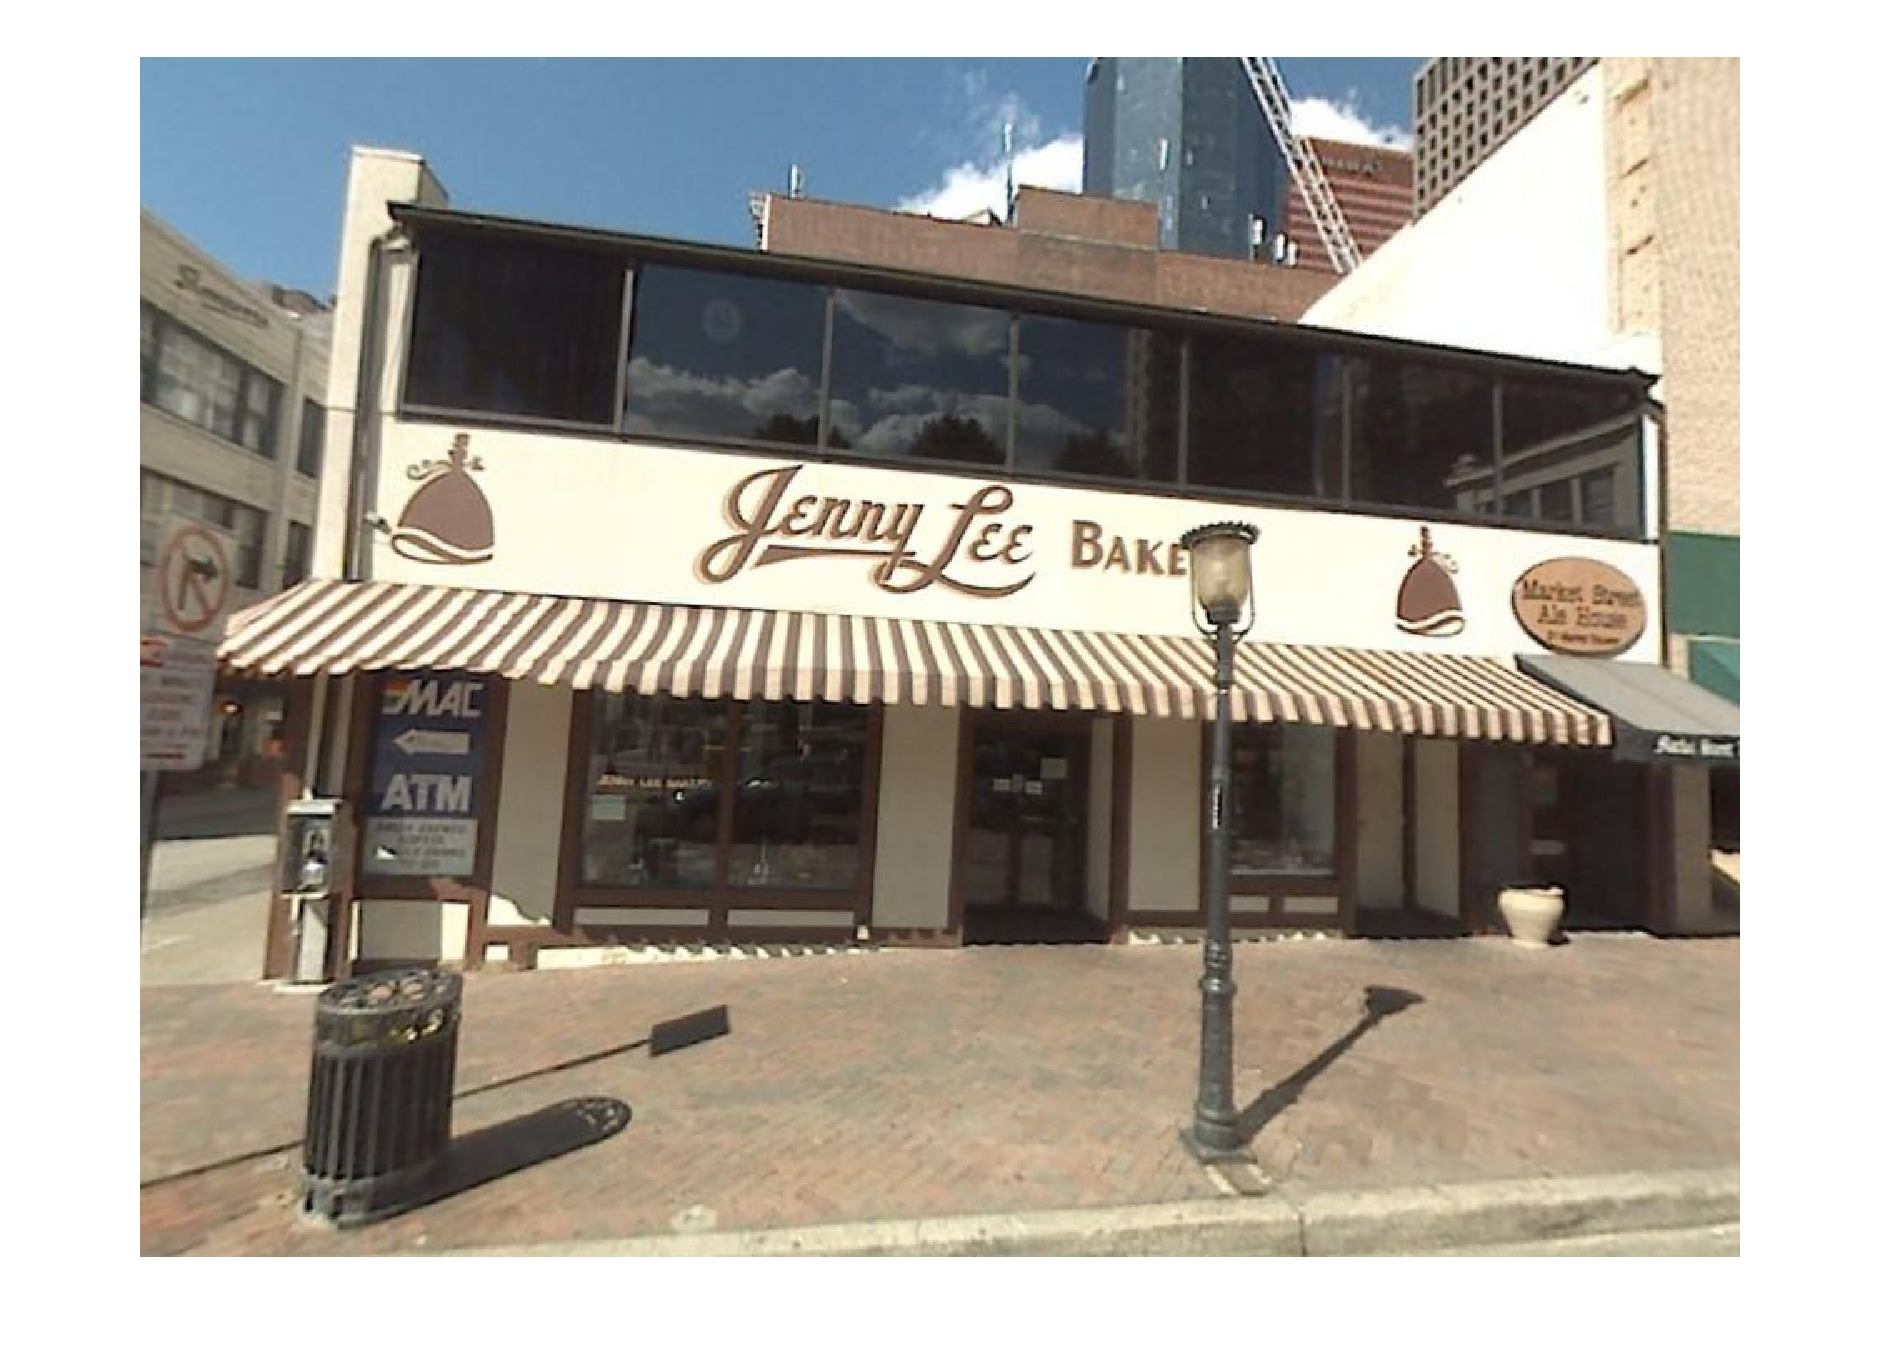
\includegraphics[width=\linewidth]{imgs/wVS3q/2882/c.jpg}
          \end{minipage} 
          \\
          \begin{minipage}{\wii}
            \centering
            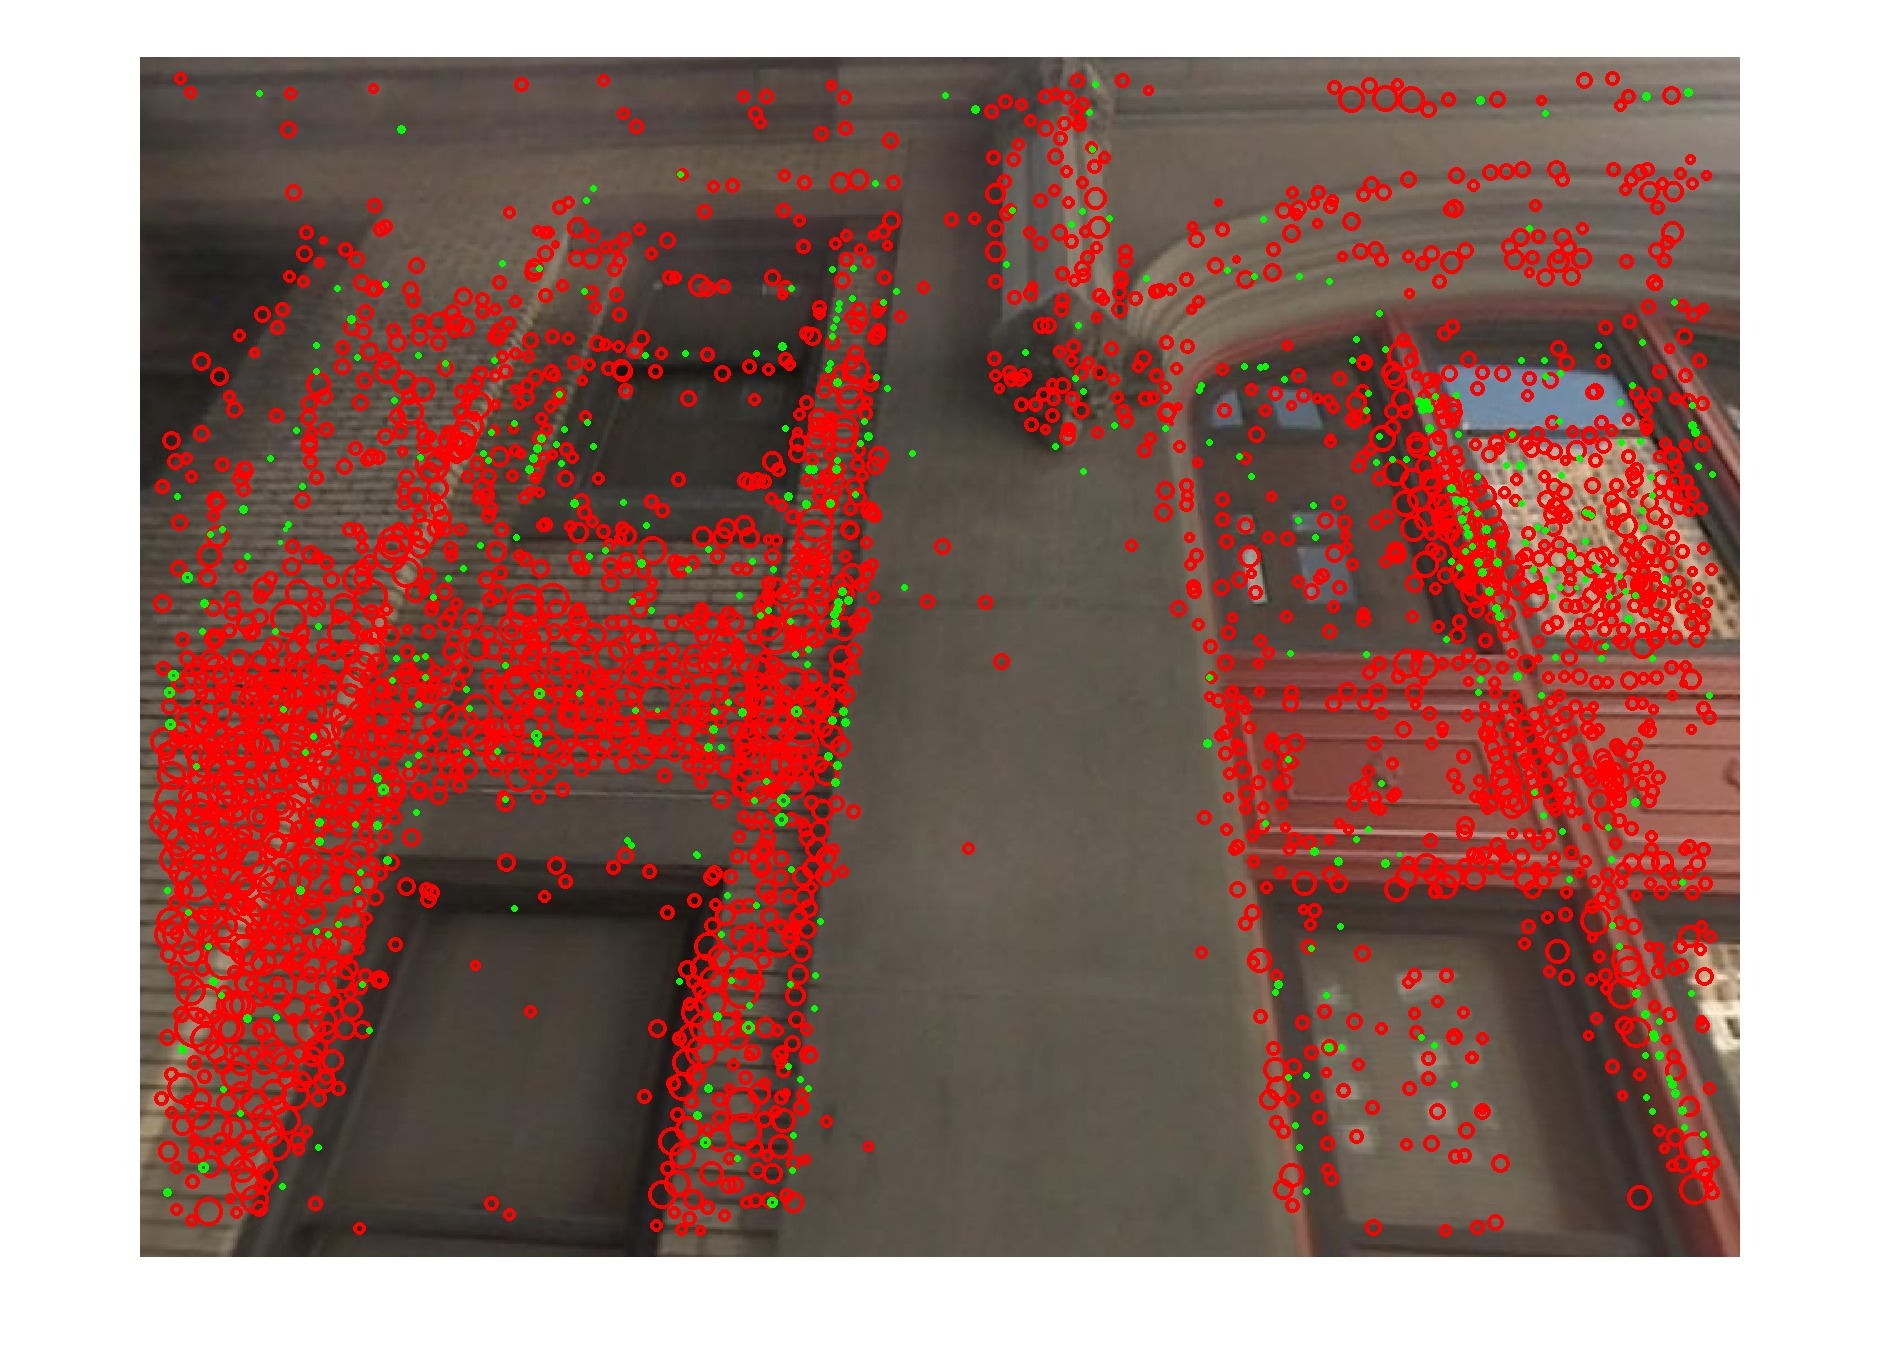
\includegraphics[width=\linewidth]{imgs/wVS3q/2882/aftrs.jpg}
            \newline
            (a)
          \end{minipage}  
          \begin{minipage}{\wii}
            \centering
            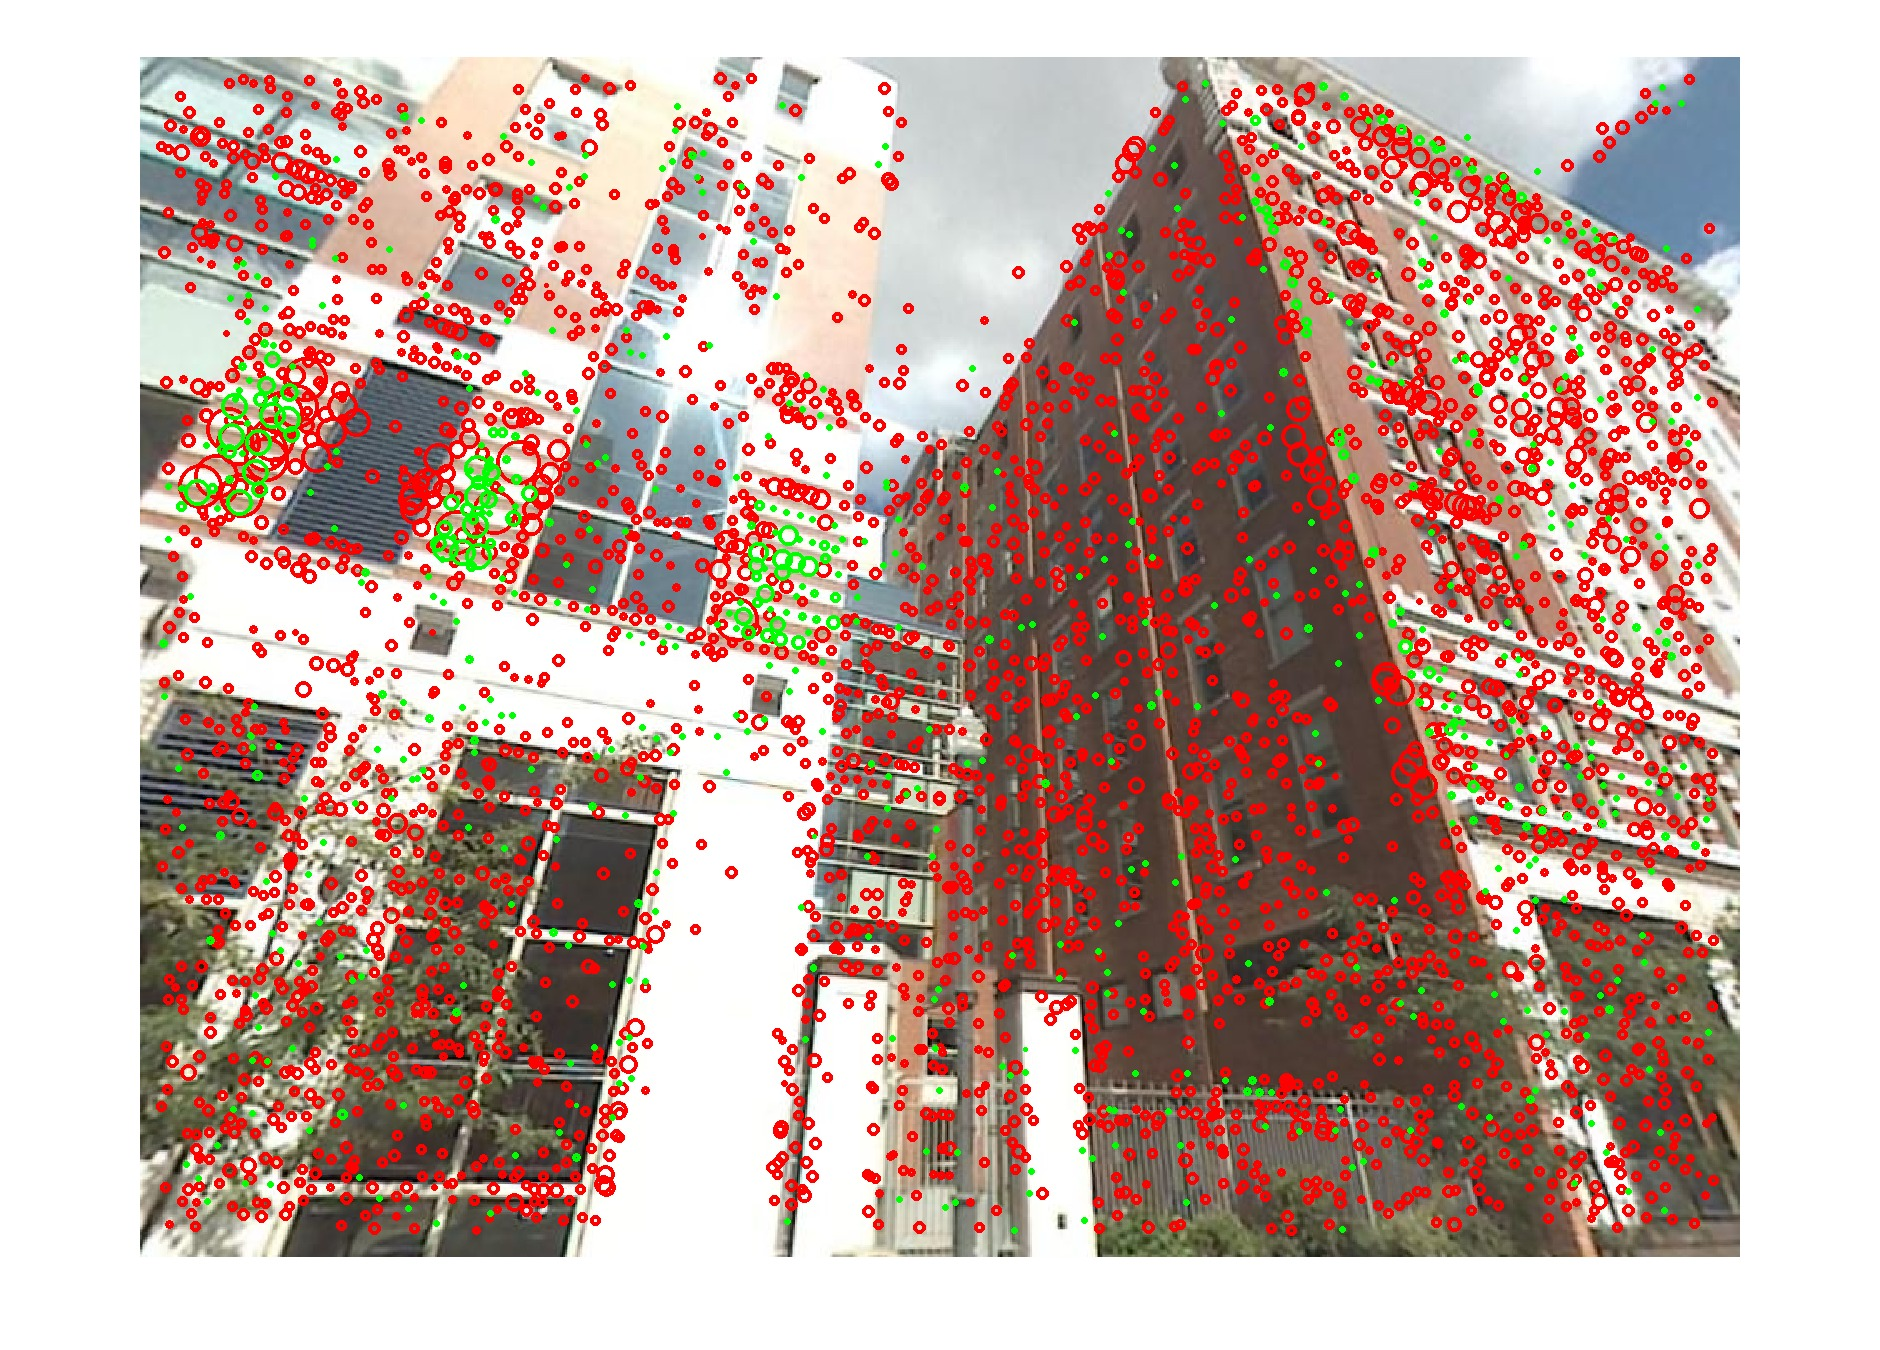
\includegraphics[width=\linewidth]{imgs/wVS3q/2882/bftrs.jpg}
            \newline
            (b)
          \end{minipage}  
          \begin{minipage}{\wii}
            \centering
            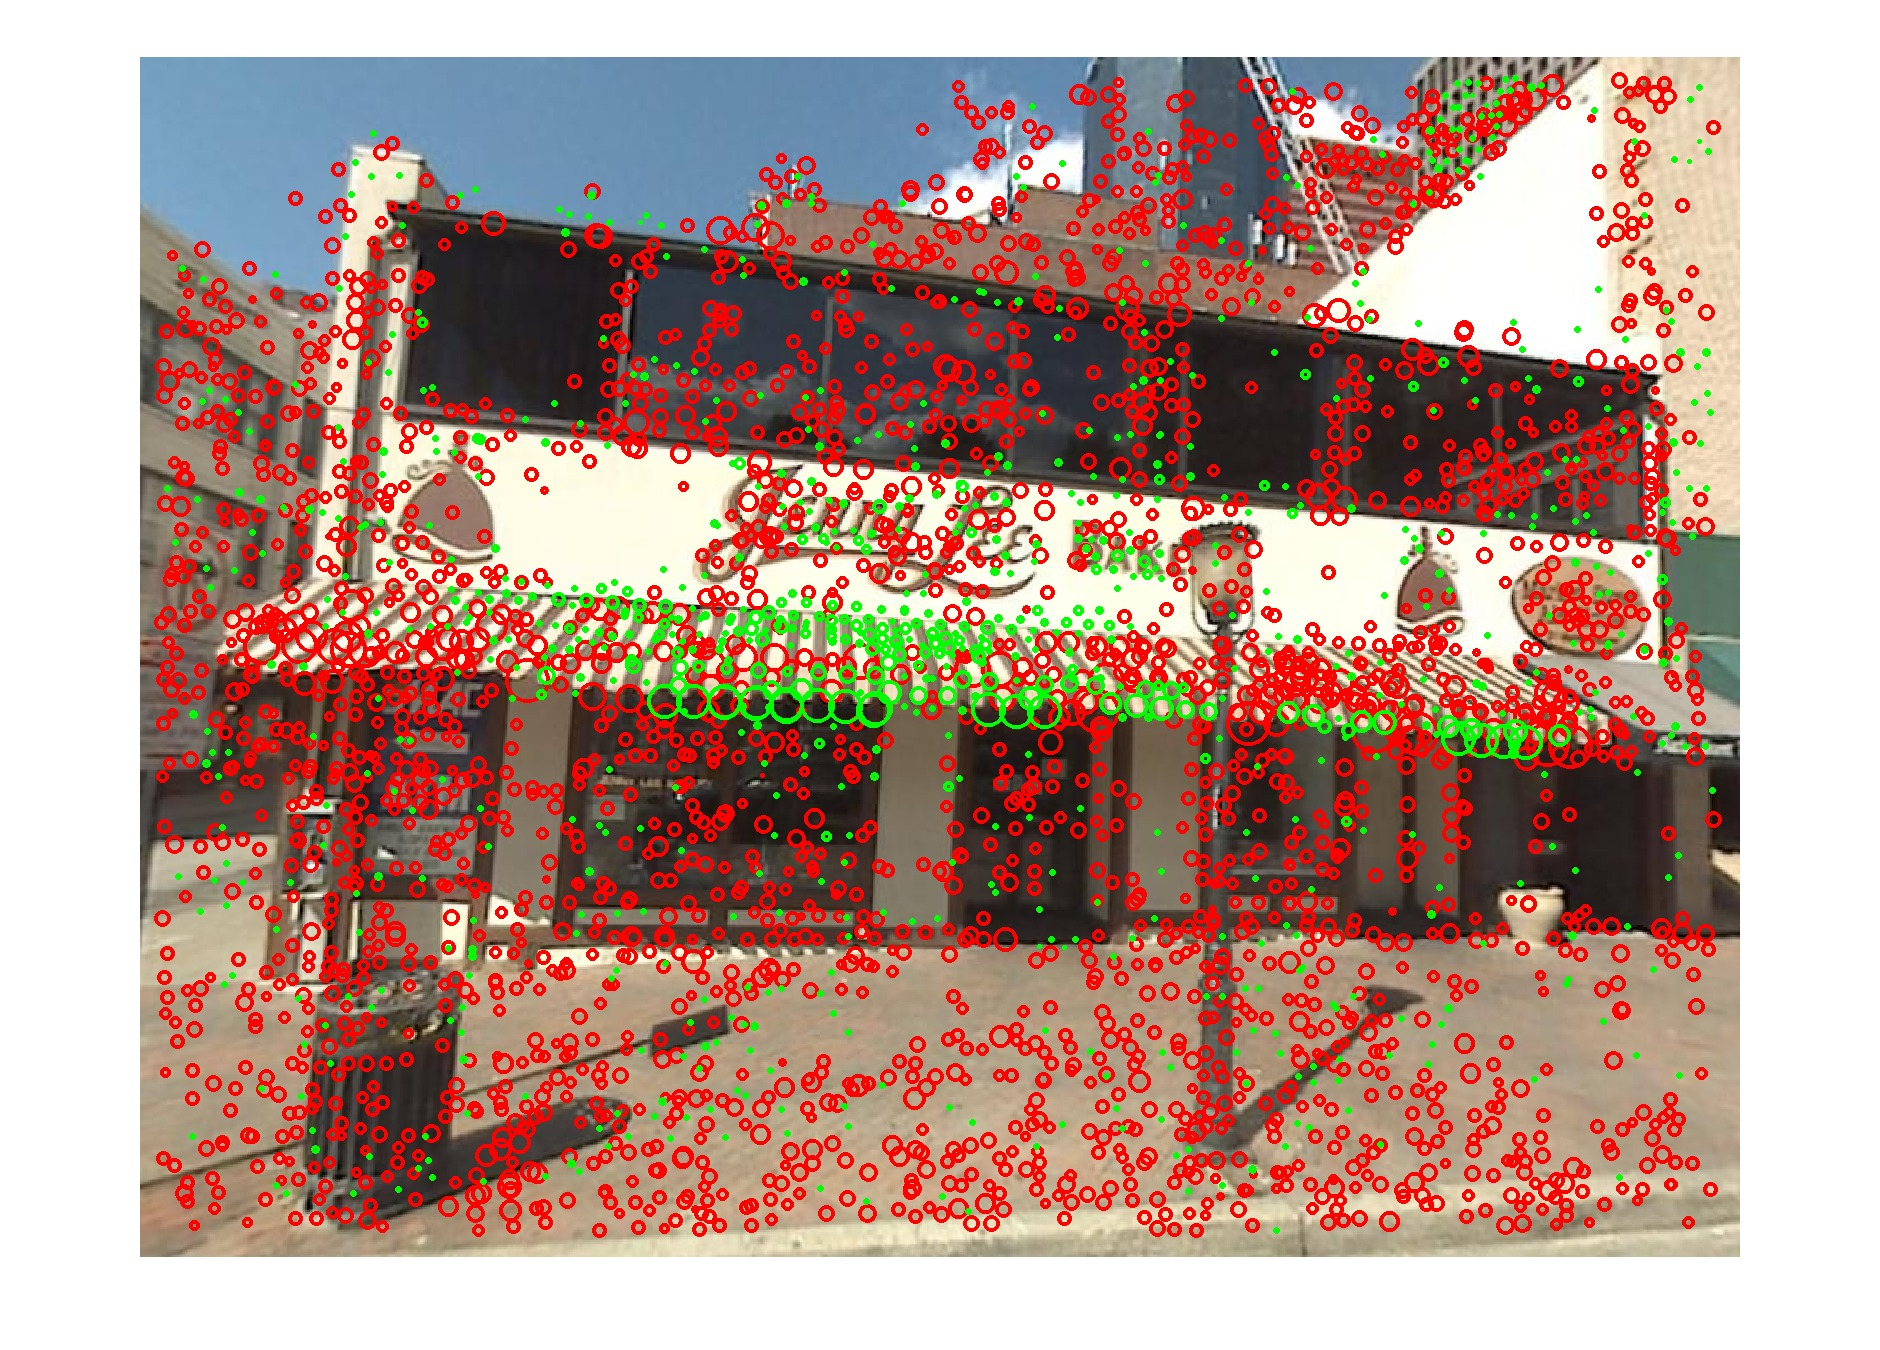
\includegraphics[width=\linewidth]{imgs/wVS3q/2882/cftrs.jpg}
            \newline
            (c)
          \end{minipage} 
    %\end{minipage}% left figure
    % %
    % %%%%%%%%%%%%%%%%%%%%%%%%%%%%%%%%%
    % \begin{minipage}{0.04\linewidth}
    %   \hspace{\linewidth}
    % \end{minipage}
    % %%%%%%%%%%%%%%%%%%%%%%%%%%%%%%%%%
    % % RIGHT FIGURE
    % \begin{minipage}{0.48\linewidth}
    %       \begin{minipage}{0.66\linewidth}
    %         \centering
    %         {\scriptsize Calibrated classifier score $f_j$}
    %         \\
    %         \vspace{2mm}
    %         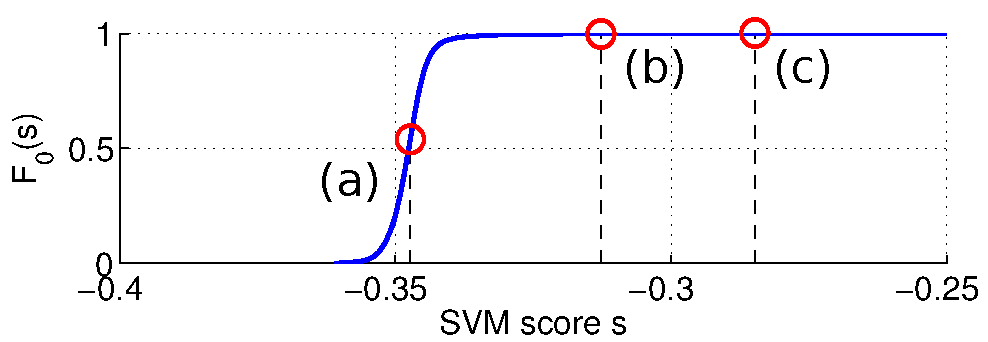
\includegraphics[width=\linewidth]{imgs/wVS3q/2932/graphBigO.pdf}
    %       \end{minipage} 
    %       %
    %       \begin{minipage}{\wii}
    %         \centering
    %         \centerline{\scriptsize Target database image $j$}
    %         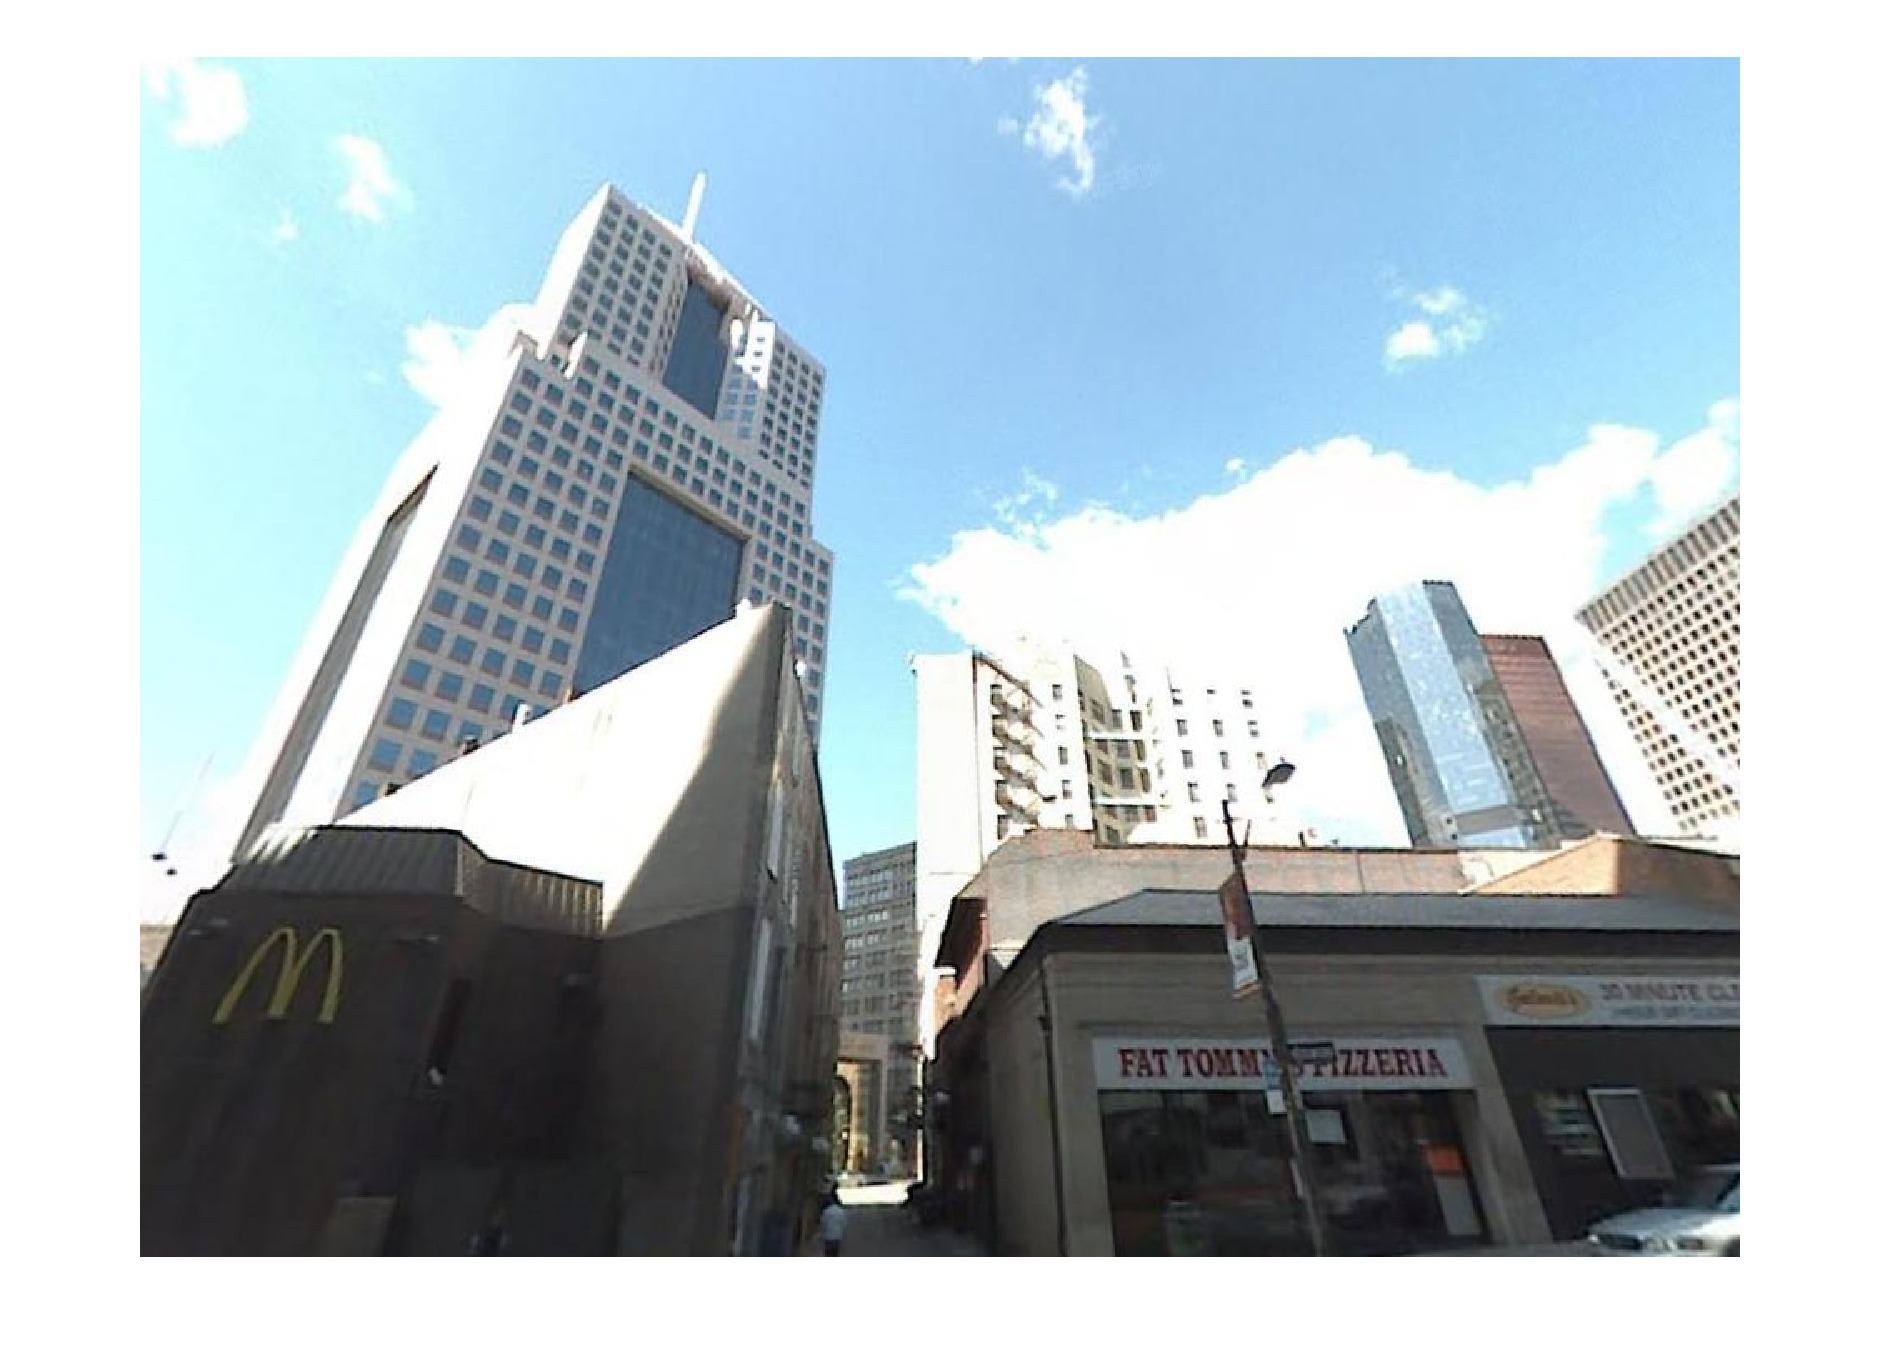
\includegraphics[width=\linewidth]{imgs/wVS3q/2932/j.jpg}
    %       \end{minipage}  
    %       \vspace{3mm}
    %       \\
    %       \centerline{\scriptsize Classified query images $f_j(q)$} 
    %       \\
    %       \begin{minipage}{\wii}
    %         \centering
    %         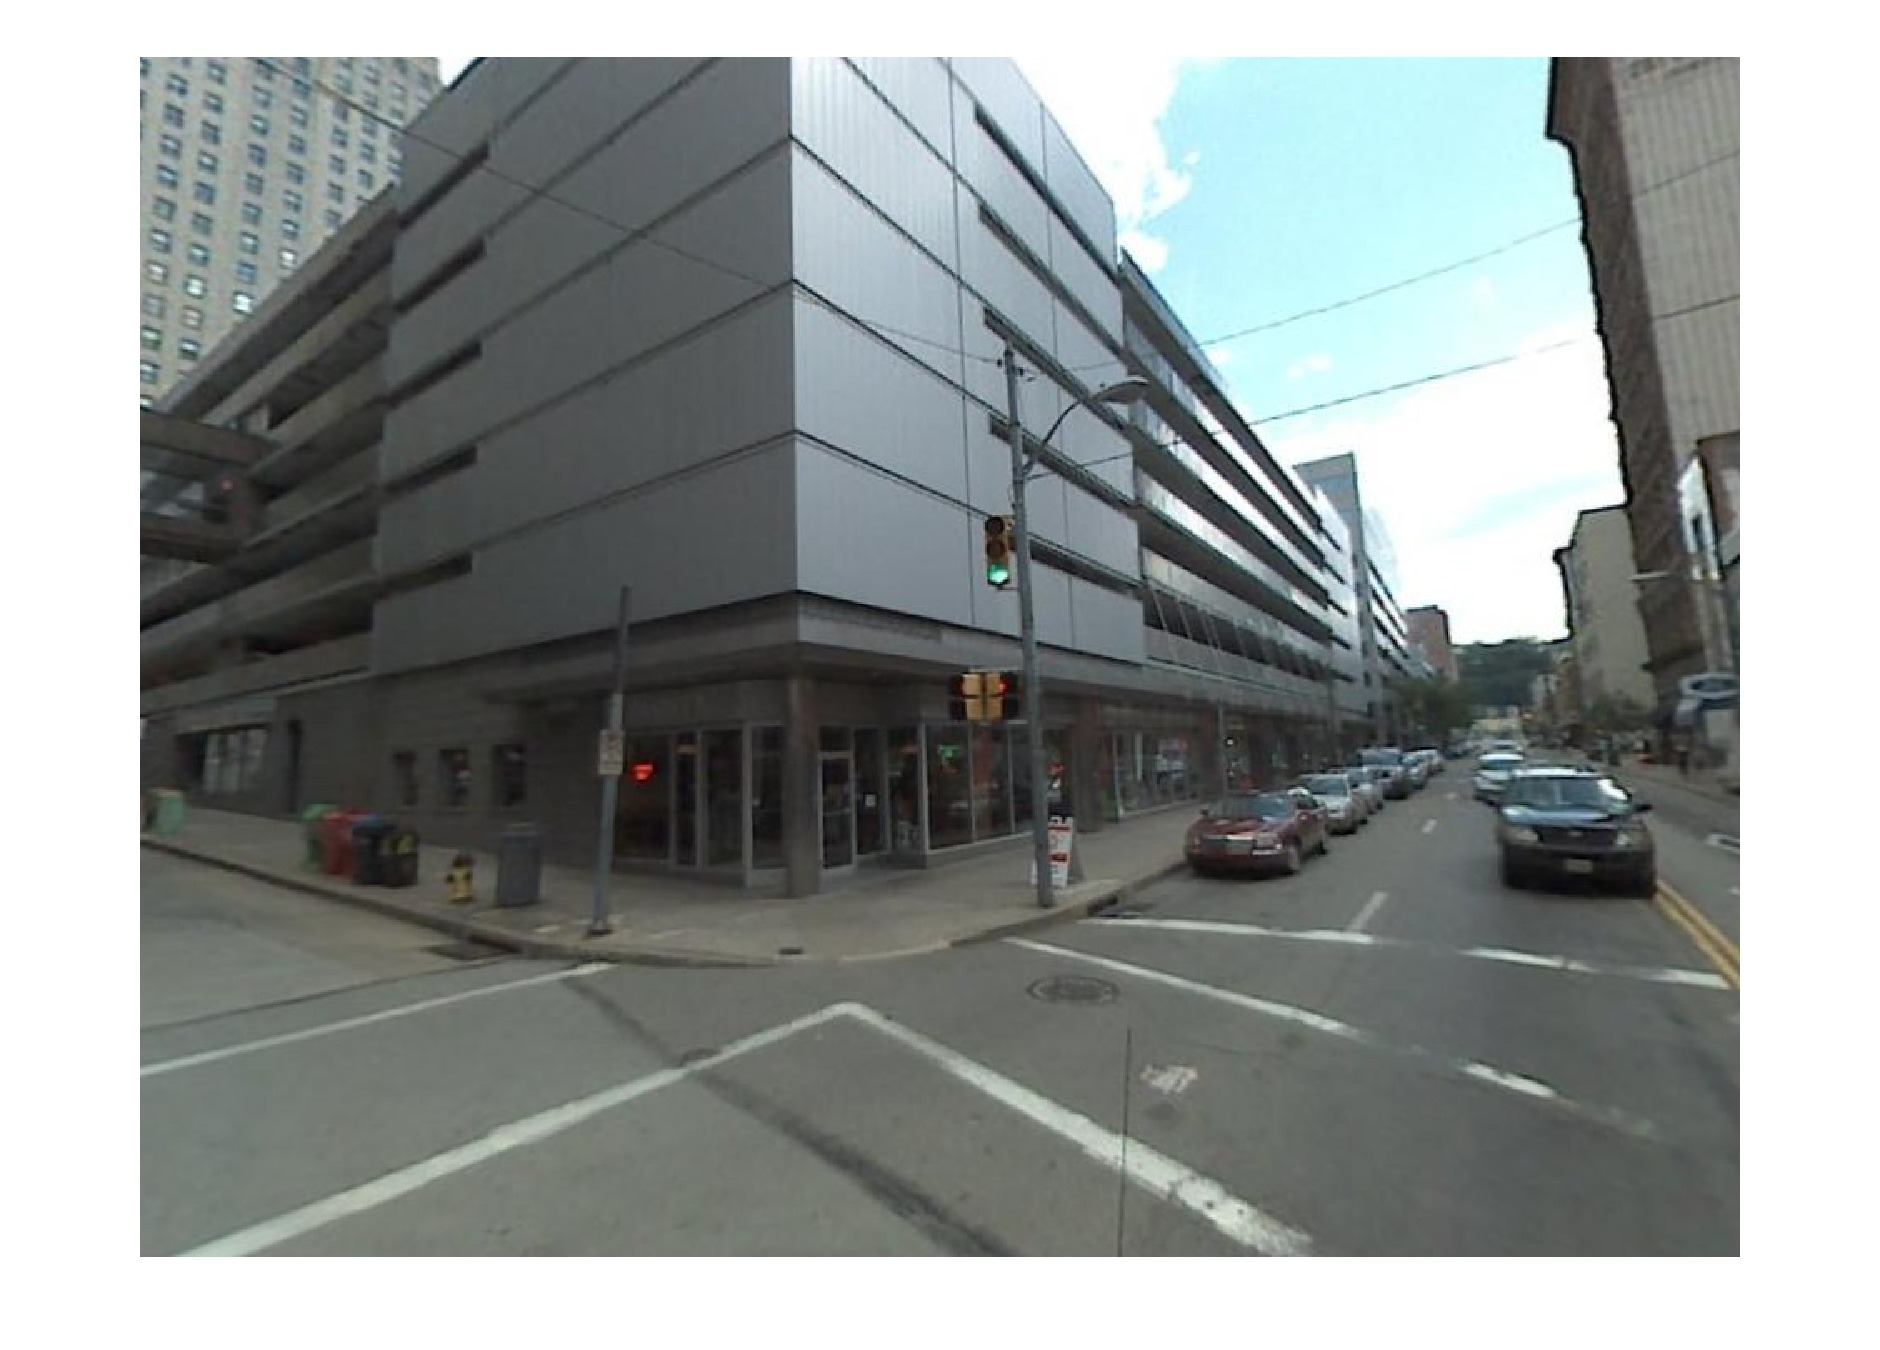
\includegraphics[width=\linewidth]{imgs/wVS3q/2932/a.jpg}
    %       \end{minipage}  
    %       \begin{minipage}{\wii}
    %         \centering
    %         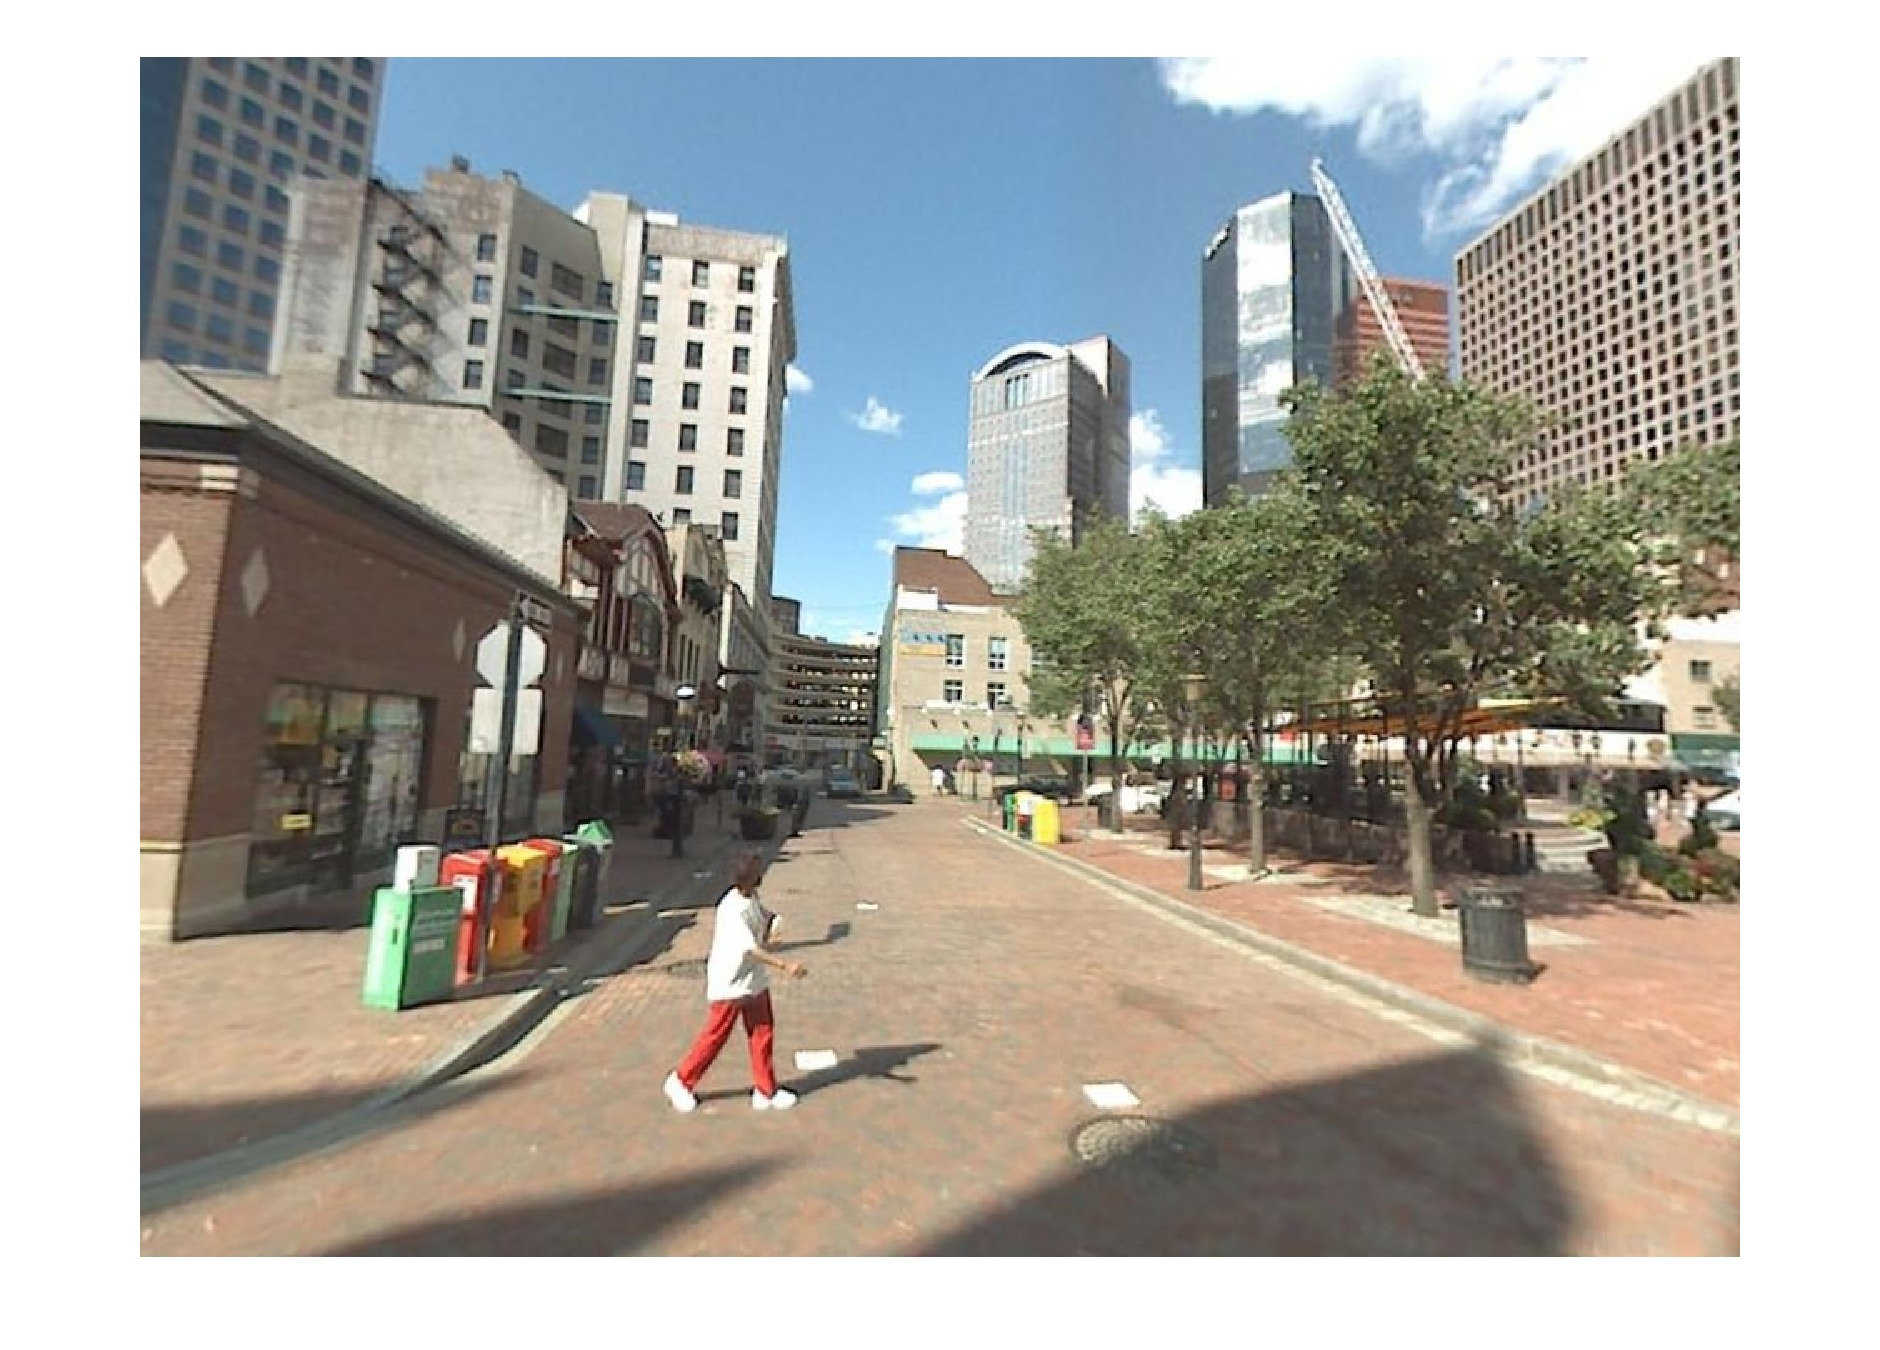
\includegraphics[width=\linewidth]{imgs/wVS3q/2932/b.jpg}
    %       \end{minipage}  
    %       \begin{minipage}{\wii}
    %         \centering
    %         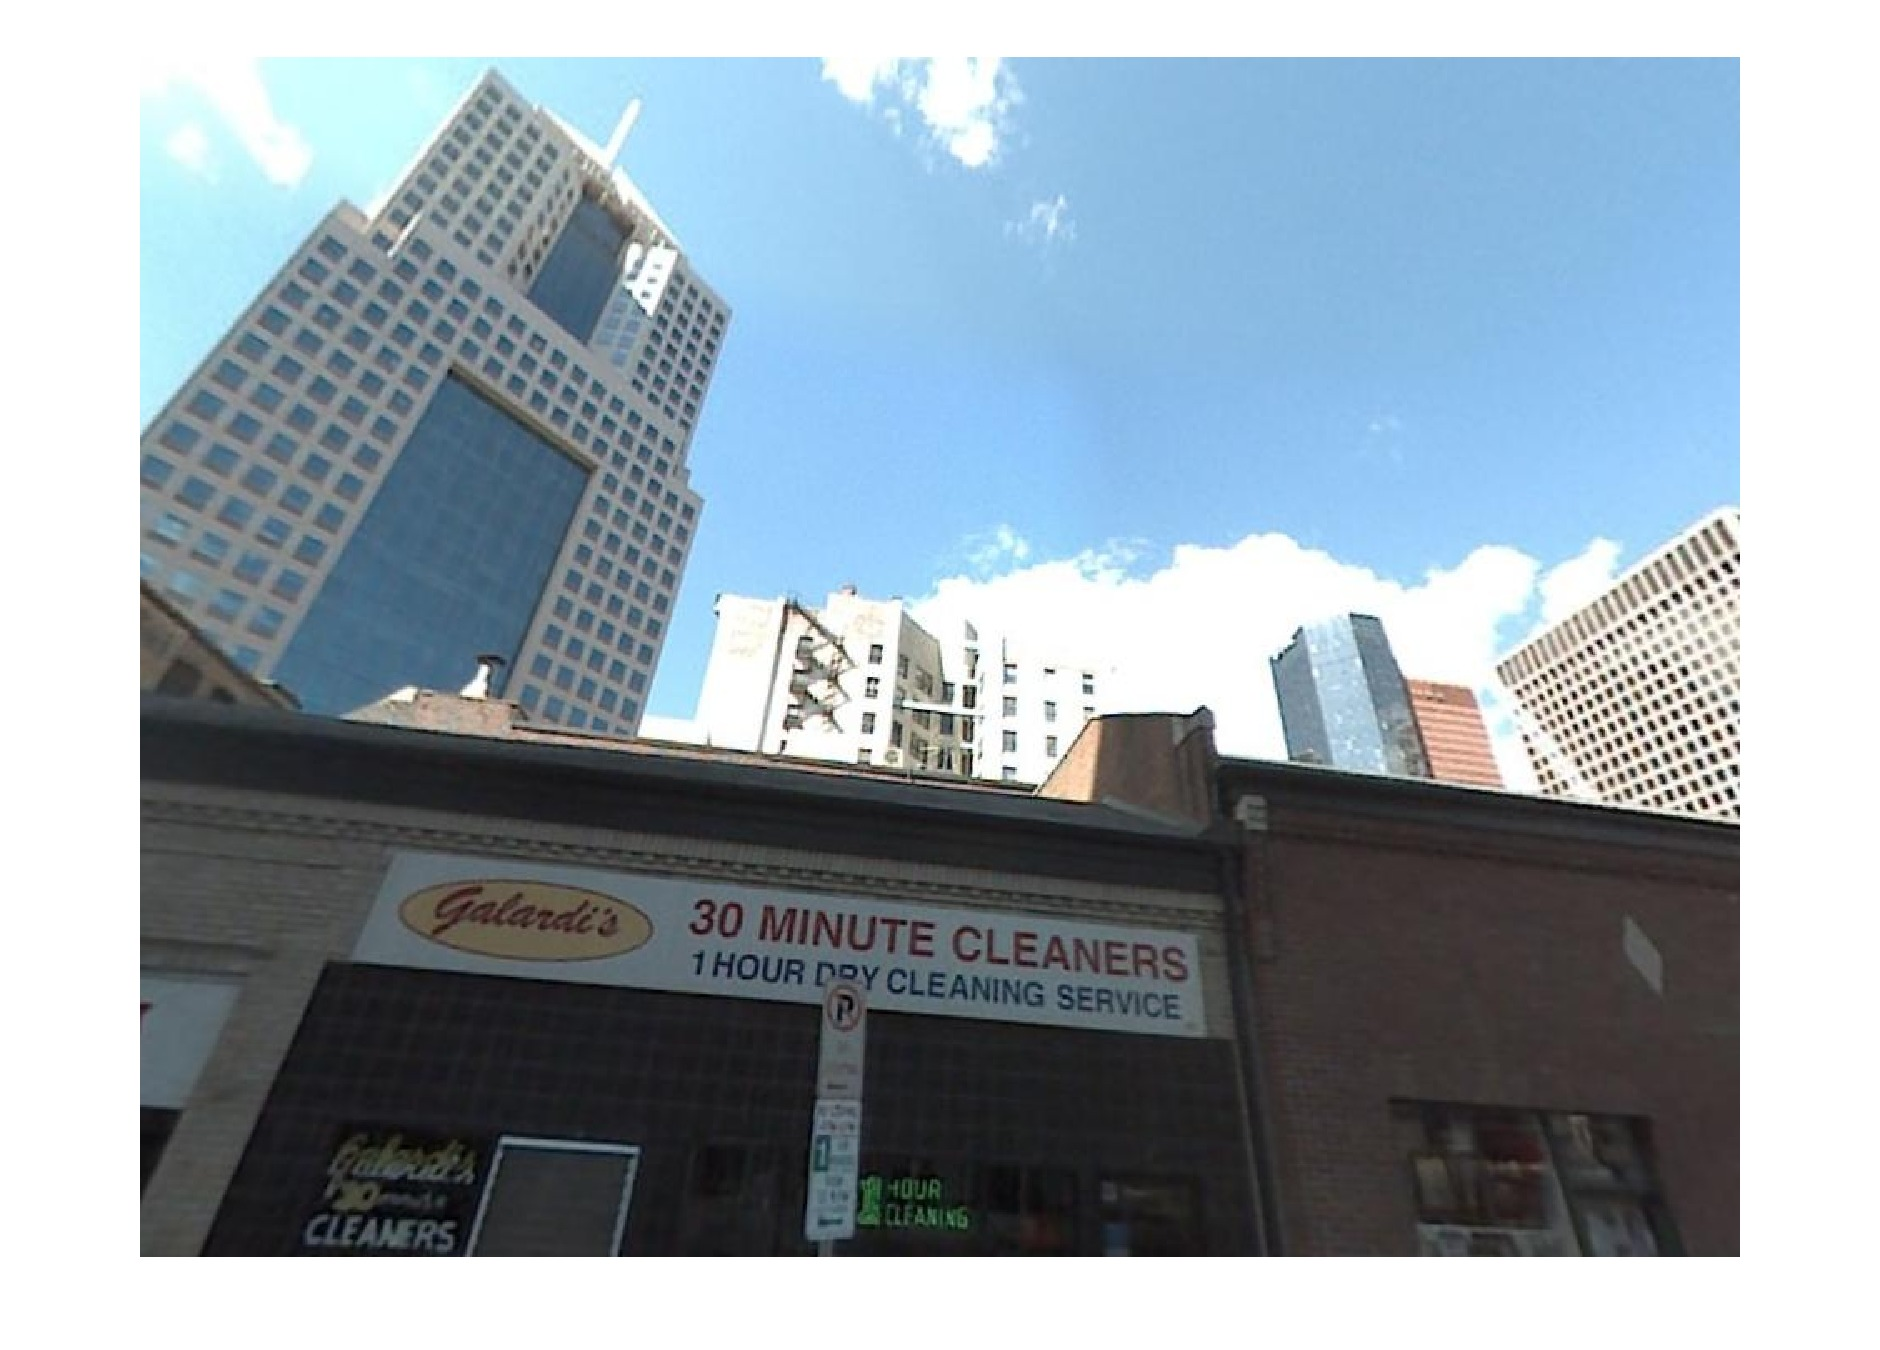
\includegraphics[width=\linewidth]{imgs/wVS3q/2932/c.jpg}
    %       \end{minipage} 
    %       \\
    %       \begin{minipage}{\wii}
    %         \centering
    %         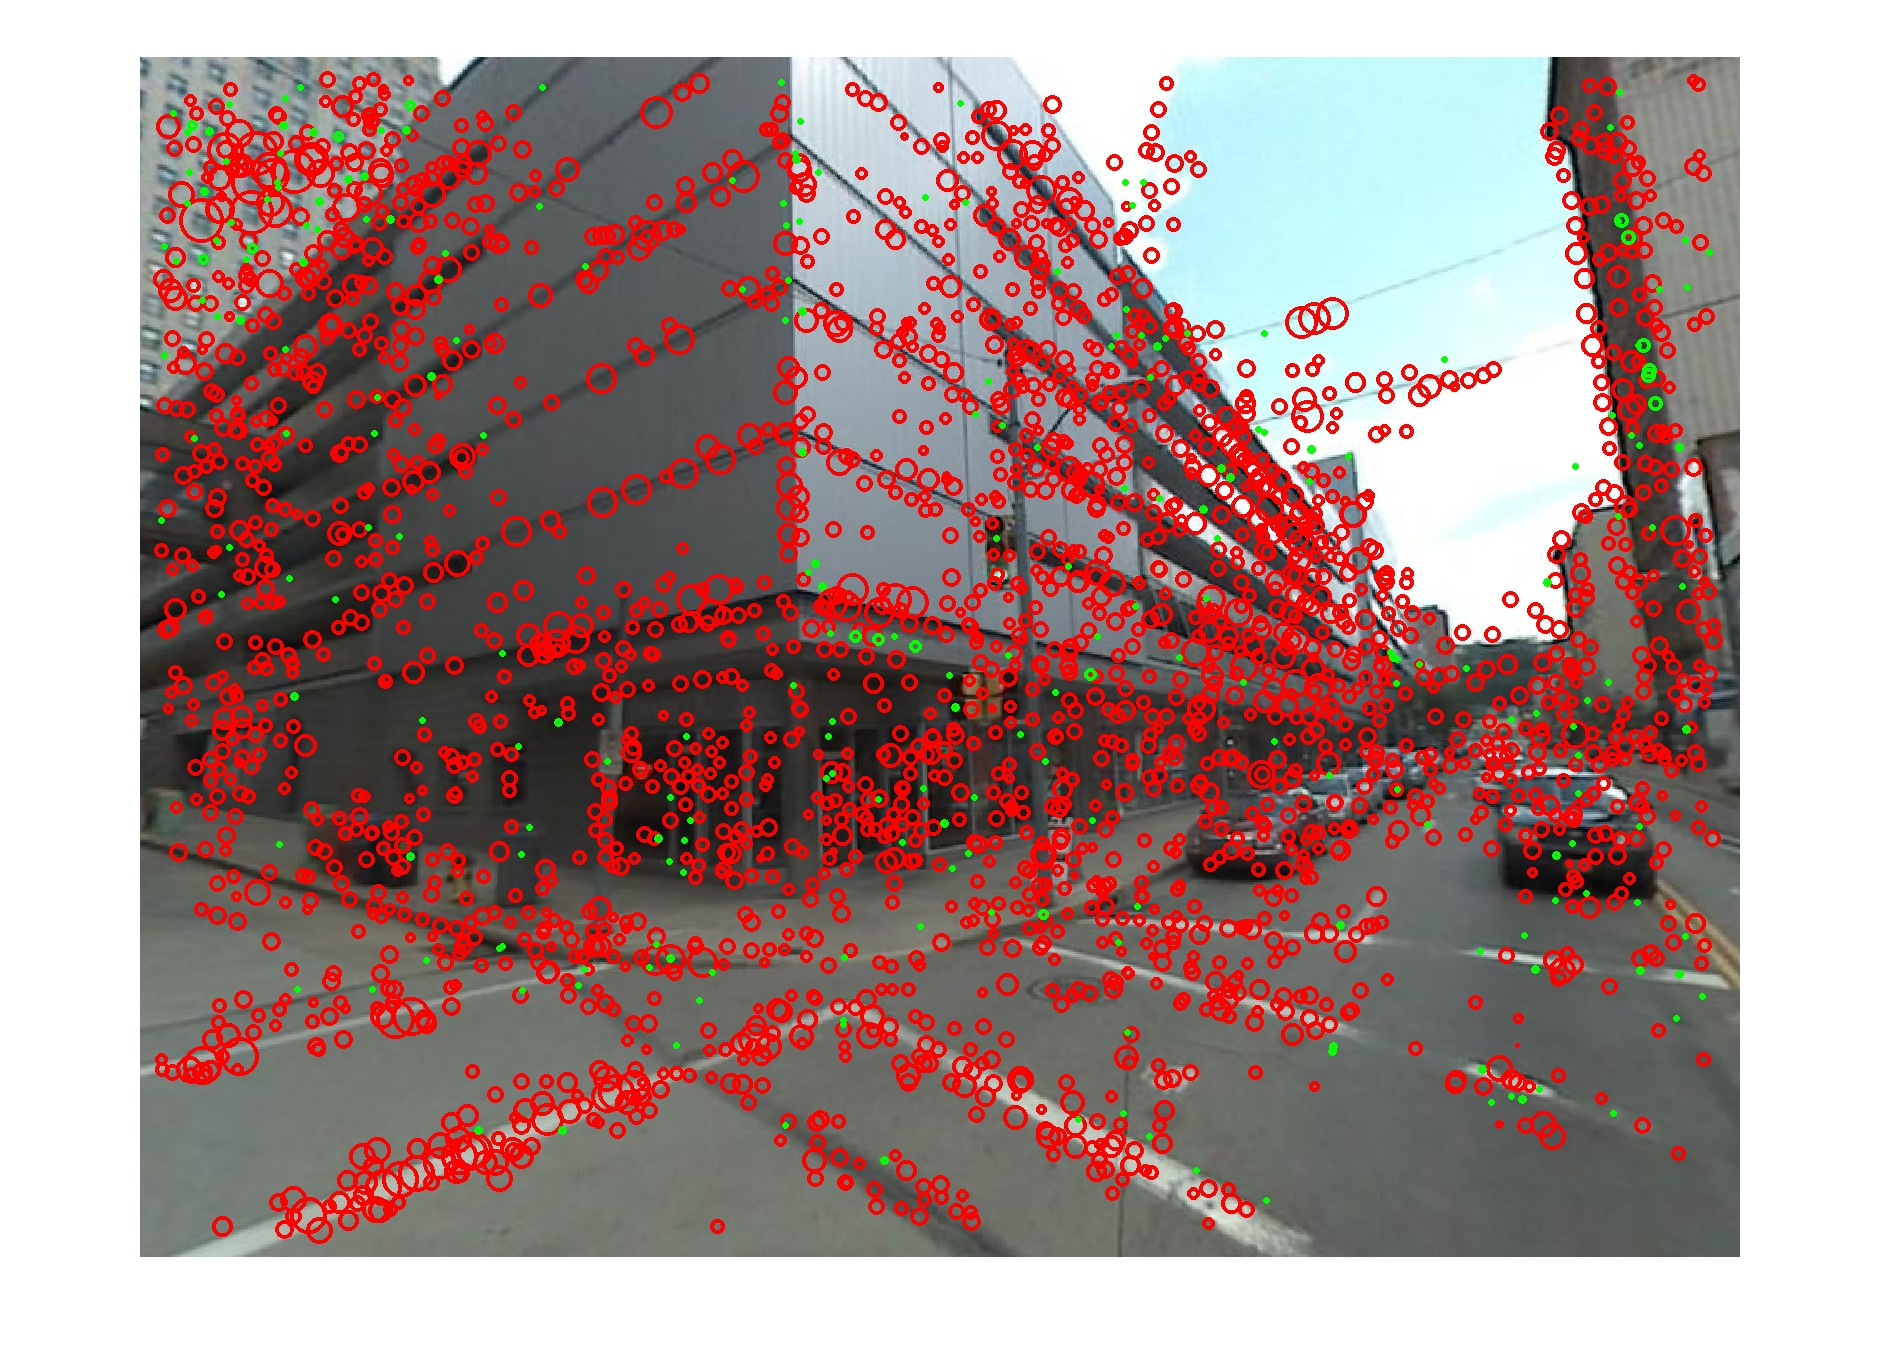
\includegraphics[width=\linewidth]{imgs/wVS3q/2932/aftrs.jpg}
    %         \newline
    %         (a)
    %       \end{minipage}  
    %       \begin{minipage}{\wii}
    %         \centering
    %         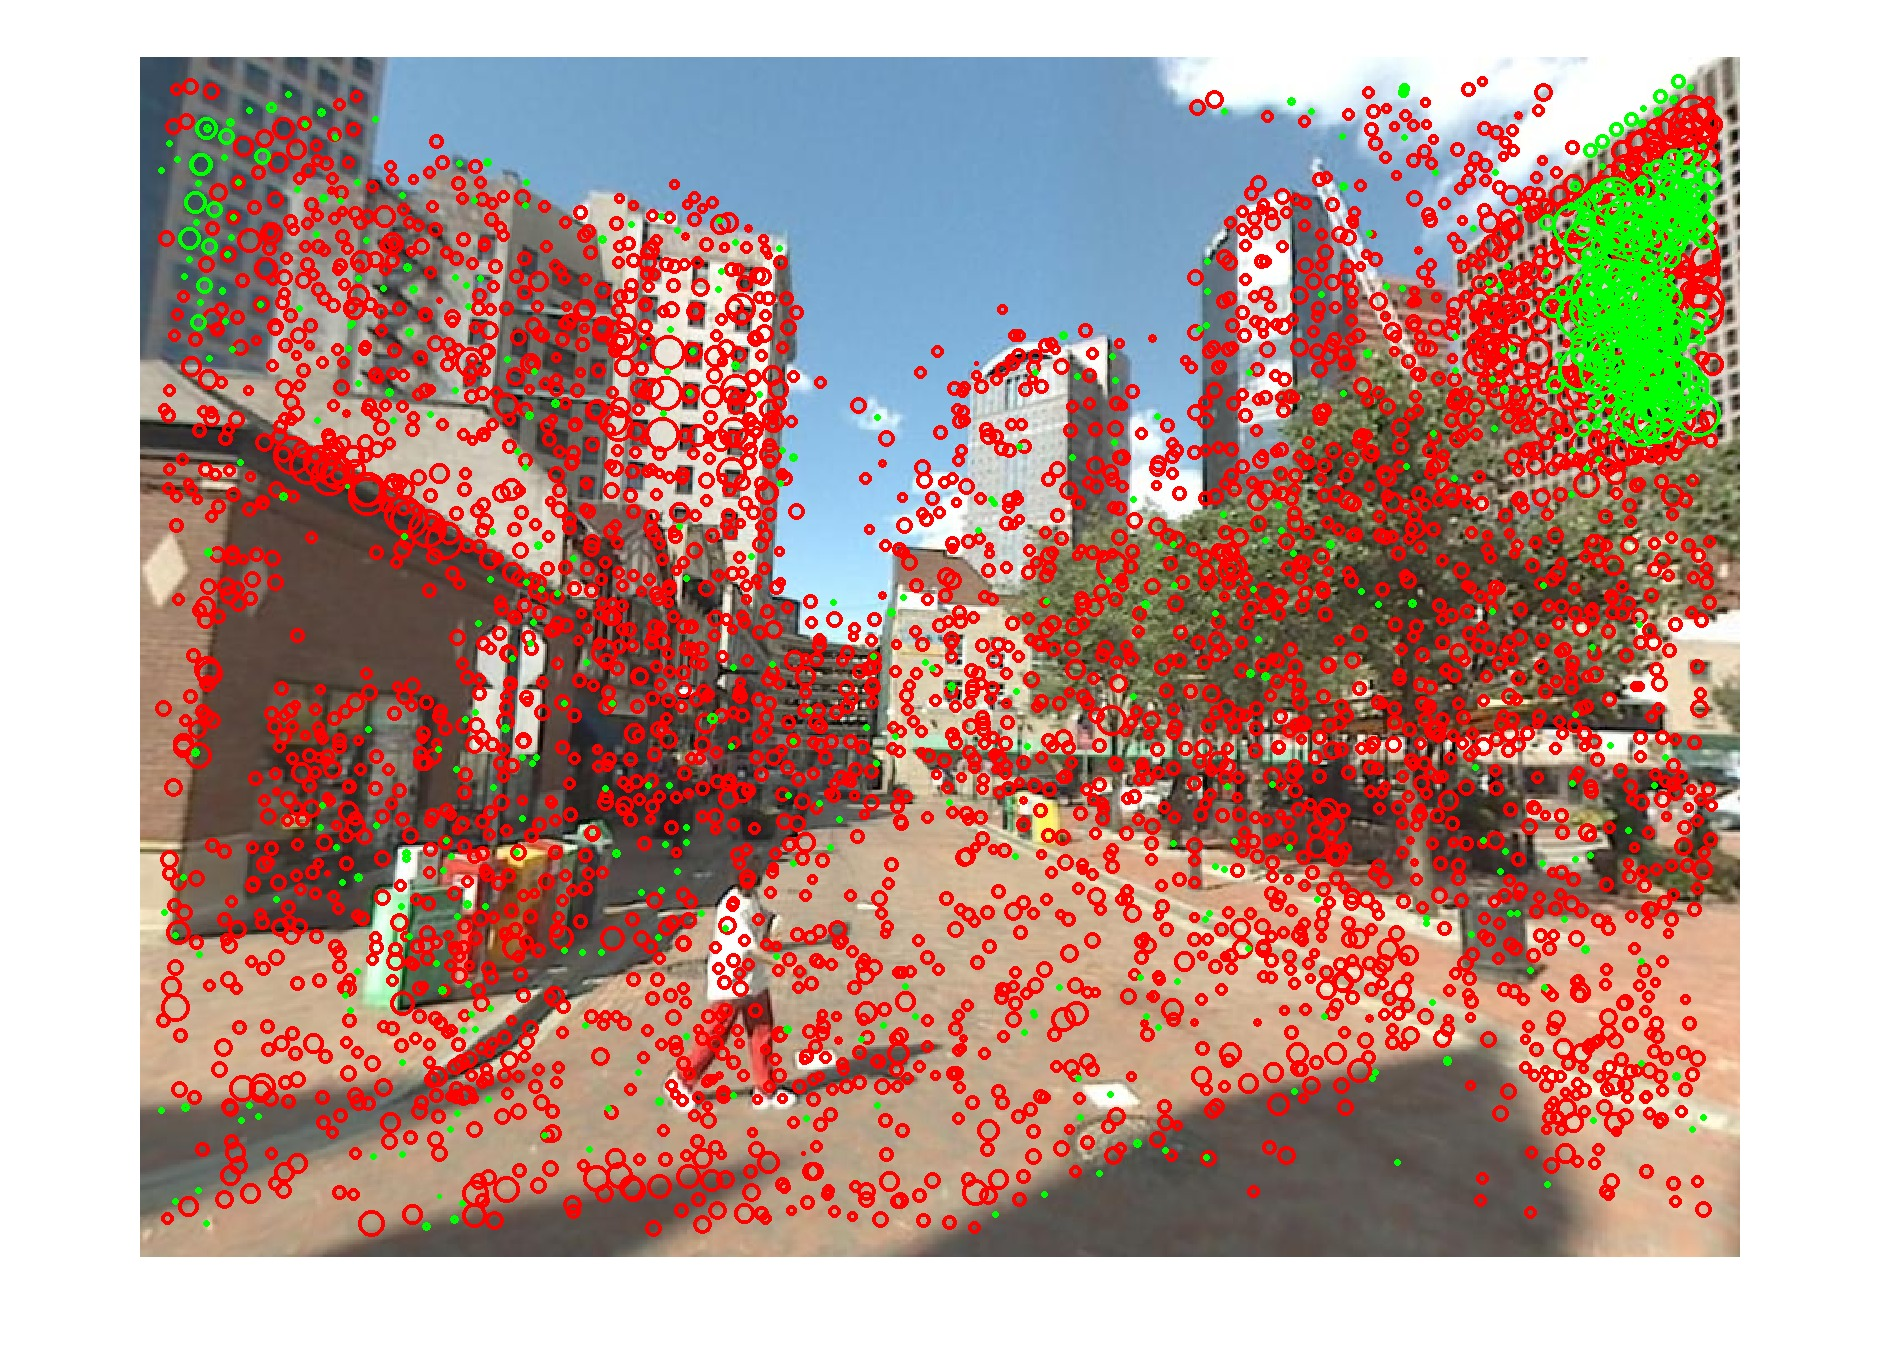
\includegraphics[width=\linewidth]{imgs/wVS3q/2932/bftrs.jpg}
    %         \newline
    %         (b)
    %       \end{minipage}  
    %       \begin{minipage}{\wii}
    %         \centering
    %         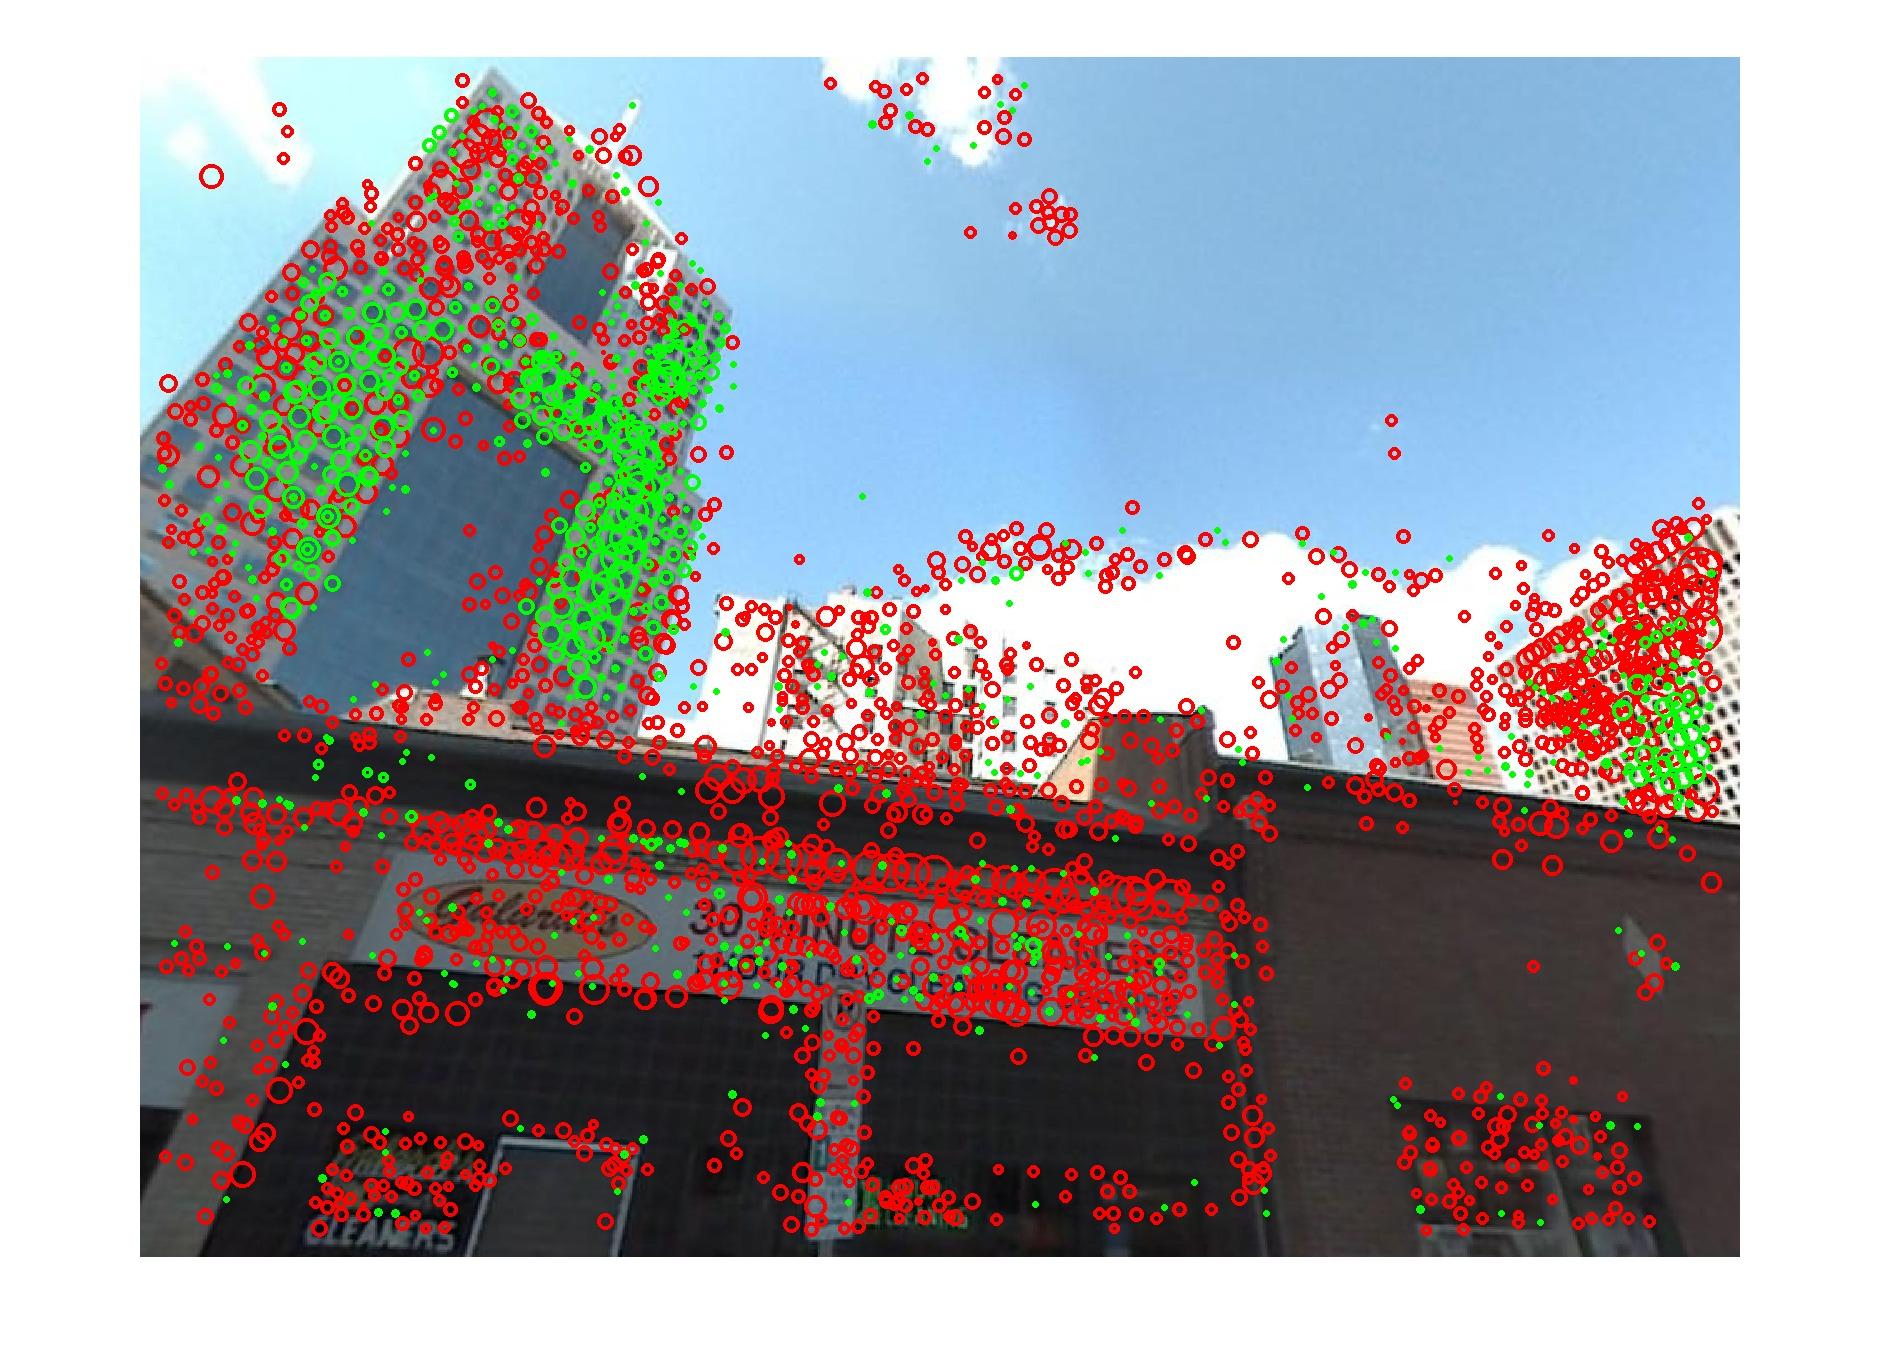
\includegraphics[width=\linewidth]{imgs/wVS3q/2932/cftrs.jpg}
    %         \newline
    %         (c)
    %       \end{minipage} 
    % \end{minipage}% right figure
    %
    %\vspace*{-2mm}
    \caption{
      {\bf  A visualization of learnt feature weights for two database images. In each panel:} 
      \emph{first~row:} 
      (Right) Target database image $j$. 
      (Left) Cumulative density function (or calibrated score) learnt for the SVM scores of the corresponding classifier $f_j$;  three query images displayed on the 
      \emph{second row} are represented by their SVM scores and cdf values $F_0(s)$, denoted (a)-(c) on the graph. 
      \emph{Third~row:} A visualization of the contribution of each feature to the SVM score for the corresponding query image. Red circles represent features with negative weights while green circles correspond to features with positive weights. The area of each circle is proportional to the contribution of the corresponding feature to the SVM score.
      %
      Notice that the correctly localized queries (c) contain more green colored features than queries from other places (b) and (a). Query (b) gets a high score because the building has orange and white stripes similar to the the sun-blinds of the bakery, which are features that also have large positive weights in the query image (c) of the correct place.
    }
    \label{fig:3qVSw}
        \vspace*{2mm}
    \end{figure*}